% =============================================================================
%  Conan — A Hallucination-Resistant RAG Pipeline for Egyptian Criminal Law
%
%  Format:  Elsevier Procedia Computer Science (matches teeem.pdf / arabicRag.pdf)
%  Engine:  XeLaTeX (required for Arabic content)
%
%  Compile:
%       xelatex research_paper.tex
%       xelatex research_paper.tex     % second pass for cross-references
%
%  Recommended workflow: upload to Overleaf, set Compiler = XeLaTeX.
% =============================================================================
\documentclass[final,1p,times]{elsarticle}

% --- Core packages -----------------------------------------------------------
\usepackage[utf8]{inputenc}
\usepackage{amsmath,amssymb,amsfonts}
\usepackage{graphicx}
\usepackage{booktabs}
\usepackage{array}
\usepackage{multirow}
\usepackage{tabularx}
\usepackage[table]{xcolor}
\usepackage[font=small,labelfont=bf,labelsep=period]{caption}
\usepackage{url}
\usepackage{hyperref}
\hypersetup{colorlinks=true,linkcolor=blue,urlcolor=blue,citecolor=blue}

% --- Publication-quality table helpers ---------------------------------------
% A light row-tint for the header band of every data table, plus a reusable
% left-aligned auto-width column type. \rowcolors is avoided (it fights
% booktabs rules); instead we tint header cells explicitly via \tabhead.
\definecolor{tabhead}{gray}{0.92}
\definecolor{tabalt}{gray}{0.97}
\newcommand{\thead}[1]{\textbf{#1}}                 % bold table-header cell
\newcolumntype{L}[1]{>{\raggedright\arraybackslash}p{#1}}
\newcolumntype{C}[1]{>{\centering\arraybackslash}p{#1}}
\newcolumntype{R}[1]{>{\raggedleft\arraybackslash}p{#1}}
\newcommand{\YES}{\textcolor{green!55!black}{\checkmark}}
\newcommand{\NO}{\textcolor{red!65!black}{\ding{55}}}
\usepackage{pifont} % \ding for cross-marks in feature tables

% --- TikZ (pipeline figure) --------------------------------------------------
\usepackage{tikz}
\usetikzlibrary{positioning,arrows.meta,shapes.geometric,calc,fit,backgrounds}

% --- Arabic support (XeLaTeX) ------------------------------------------------
% Compiling with pdfLaTeX will not render Arabic glyphs — use XeLaTeX.
% NOTE: we deliberately avoid polyglossia/bidi here. The document only contains
% short inline Arabic snippets (via \ar{...}); polyglossia's \setotherlanguage
% {arabic} loads the bidi package, which is incompatible with elsarticle's
% \maketitle and crashes the front matter. Instead we shape inline Arabic with
% fontspec and obtain correct right-to-left ordering via XeTeX's native
% TeX--XeT primitives (\TeXXeTstate + \beginR/\endR), which build cleanly under
% stock XeLaTeX / tectonic / Overleaf.
\usepackage{fontspec}
\newfontfamily{\arabicfont}[Script=Arabic]{Amiri}
\TeXXeTstate=1
\newcommand{\ar}[1]{{\arabicfont\beginR #1\endR}}

% --- Elsevier Procedia front-matter housekeeping -----------------------------
\journal{Procedia Computer Science}

% \dochead is provided by Elsevier's Procedia author kit (ecrc.sty). Guard it so
% the manuscript also compiles under stock elsarticle / XeLaTeX / tectonic; the
% \providecommand is a no-op when the real Procedia style is loaded.
\providecommand{\dochead}[1]{}

\begin{document}

\begin{frontmatter}

% Conference banner (mirrors the Procedia ACLing style of [1] and [5])
\dochead{International Conference on AI in Computational Linguistics}

\title{Conan: A Hallucination-Resistant, Agentic Retrieval-Augmented
Generation Framework for Arabic Legal Reasoning in Egyptian Criminal Law}

% Authors --------------------------------------------------------------------
\author[a]{Mirna Nageh\corref{cor1}}
\ead{mirnanagehb.w@gmail.com}
\author[a]{Wageh Mostafa}
\author[a]{Seif Sherif}
\author[a]{Mariam Mohamed}
\author[a]{Mayar Mohammed}

\address[a]{Faculty of Computers \& Artificial Intelligence, Capital (Helwan) University, Egypt}

\cortext[cor1]{Corresponding author.}

% Abstract -------------------------------------------------------------------
\begin{abstract}
Retrieval-Augmented Generation (RAG) has emerged as the dominant architecture
for grounding large language models on domain knowledge, yet its application
to Arabic legal information retrieval continues to suffer from hallucinated
statutory citations and confabulation when retrieval surfaces topically-related
but legally-inadequate context. We present \textbf{Conan}, a production-grade
Arabic legal assistant for the Egyptian Criminal Code (\ar{قانون العقوبات})
and the Code of Criminal Procedure (\ar{قانون الإجراءات الجنائية}). Our
contribution is twofold. First, we describe the construction of an Egyptian
criminal-law corpus assembled from scratch: 933~legacy-format source files
(818~\texttt{.doc}, 112~\texttt{.pdf}, 3~\texttt{.docx}) gathered from
authoritative Egyptian legal collections, manually OCR-processed and cleaned
into 1{,}057 UTF-8 documents and indexed as 47{,}028 chunks. The resulting
dataset is released publicly on HuggingFace as
\emph{Egyptian\_Criminal\_Legal\_Assistant\_RAG\_V2}. Second, we introduce a
seven-layer grounding-defence pipeline---input gating, citation-grounding
prompts with substantive-vs-procedural law disambiguation, evidence
validation, corrective retry with a block-list, an article-lookup rescue
indexing 1{,}494 distinct statutory articles, iterative retrieval with
adaptive $k$-expansion, and deterministic answer post-processing---layered on
top of a hybrid retrieval baseline (FAISS + BM25 + Reciprocal Rank Fusion +
cross-encoder reranking). On a 28-question Arabic legal benchmark spanning
substantive and procedural questions, the complete system reduces the
hallucinated-citation rate from a baseline of 28.6\,\% to \textbf{0.0\,\%} and
the evidence-validation pass rate from 71.4\,\% to \textbf{100\,\%}. We also
report a negative result on synonym-based query expansion. Beyond
single-question Q\&A, the system escalates open-ended case work to a
\textbf{six-stage multi-agent agentic pipeline}---document analysis, weakness
detection, per-weakness legal-research and precedent retrieval, defence-strategy
ranking, and grounded synthesis---in which a deterministic, code-computed timing
verdict is injected as a hard fact to eliminate a recurring chronological-reasoning
error, every argument is anchored to retrieved authority rather than parametric
memory, and a draft\,$\rightarrow$\,verify\,$\rightarrow$\,revise self-check closes the
argument-level hallucination gap; the pipeline degrades gracefully to a single-shot
path on any agent failure. The system is deployed as a production FastAPI service
with a five-provider, multi-key failover chain, big-context routing, a zero-token
answer cache, an in-process rate gate, a wall-clock cascade budget, persistent
multi-turn sessions with compaction, token streaming, automated watch-folder
ingestion with hot-reload, and a documented .NET integration contract. Finally, we report a retrieval-quality optimisation
phase targeting the retrieval ceiling that bounds answer correctness---article-aware
chunking that keeps each statute article intact in one retrievable unit (live), a
widened cross-encoder candidate pool (live), and a BGE-M3 embedding upgrade
prepared behind configuration---together with a scored evaluation harness reporting
recall@k, article-recall, primary-hit@k, MRR, hallucination rate, abstention, and
confidence calibration over a labeled gold set, so every change is measurable. We
also report a practical systems finding: on CPU-only hardware the highest-quality
embedder can be infeasible to \emph{build} without accelerator access, making the
embedder a joint quality/operability choice. We release the corpus, the system,
the multi-version evaluation trail, and the evaluation harness.
\end{abstract}

\begin{keyword}
Arabic NLP \sep Retrieval-Augmented Generation \sep Agentic AI \sep
Multi-Agent Systems \sep Legal Information Retrieval \sep Hallucination
Mitigation \sep Egyptian Criminal Law \sep Article-Lookup Rescue \sep
Iterative Retrieval \sep Article-Aware Chunking \sep BGE-M3 \sep
Neuro-Symbolic Reasoning \sep Dataset Construction
\end{keyword}

\end{frontmatter}

% =============================================================================
\section{Introduction}\label{sec:intro}

The Arabic language is spoken by approximately 422~million people across more
than twenty sovereign states, yet it remains comparatively under-served by
modern natural language processing (NLP) systems~\cite{elbeltagy2024}. This
under-representation is especially acute in \emph{Arabic legal} NLP, where
Modern Standard Arabic (MSA), domain-specific terminology, dialectal
variation, and the morphological richness of the language compound the
standard challenges of grounded language modelling.

Retrieval-Augmented Generation (RAG) has become the dominant architecture for
closing the gap between a frozen LLM's parametric memory and the dynamic,
citation-heavy demands of legal practice. By retrieving relevant passages
from a curated corpus and conditioning the generator on those passages, RAG
can in principle produce answers that are both fluent and
traceable~\cite{hrimech2025,miniraq}. However, recent surveys of Arabic legal
RAG---including the Moroccan family-code study of Hrimech et~al.\cite{hrimech2025}
and the morphologically-aware retrieval study of Aboasal et~al.\cite{aboasal2025}---identify
a recurring failure pattern: the LLM remains liable to \emph{hallucinate
statutory citations}, even when grounded retrieval is available, particularly
when the user's question maps to articles that were not surfaced in the
retrieval top-$k$.

This work makes two complementary contributions. We first describe the
\emph{construction of an Egyptian criminal-law corpus from scratch}: 933
legacy-format source files (overwhelmingly \texttt{.doc} legacy binaries
requiring manual OCR) gathered from authoritative collections of Egyptian
legal text and processed into a clean 1{,}057-document corpus, released
publicly on HuggingFace as \emph{Egyptian\_Criminal\_Legal\_Assistant\_RAG\_V2}.
We then present \textbf{Conan} (\ar{كونان}), a hallucination-resistant Arabic
legal-AI assistant built on top of this corpus. Conan layers a six-mechanism
grounding-defence pipeline on top of a standard hybrid-retrieval architecture
(FAISS dense embeddings + BM25 sparse search, fused via Reciprocal Rank
Fusion, with cross-encoder reranking). We argue---and our evaluation
empirically demonstrates---that \emph{no single technique} is sufficient for
hallucination suppression in Arabic legal RAG; a layered approach combining
input filtering, prompt engineering, post-hoc validation, article-level
metadata lookup, and answer rewriting is required.

\subsection{Contributions}

\begin{enumerate}
  \item A publicly-released Egyptian-criminal-law corpus, manually
        OCR-processed from 818 legacy \texttt{.doc} binaries and 112 PDFs into
        1{,}057 UTF-8 documents covering the Penal Code, the Code of Criminal
        Procedure, cassation rulings, criminal-law treatises, and forensic
        medicine references (Section~\ref{sec:dataset}).
  \item A \textbf{multi-stage grounding-defence pipeline}
        (Section~\ref{sec:defence}) reducing the hallucinated-citation rate
        from 28.6\,\% to 0.0\,\% on our benchmark---an absolute reduction of
        28.6 percentage points and an 8-fold relative improvement.
  \item An \textbf{article-lookup rescue subsystem} (Section~\ref{sec:rescue})
        that indexes 1{,}494 distinct Egyptian-law article numbers from chunk
        metadata at startup and uses them as a deterministic second-chance
        grounding source when post-generation evidence validation flags a
        missing citation.
  \item \textbf{Iterative retrieval with adaptive $k$-expansion}
        (Section~\ref{sec:iter}) that widens retrieval to $k\!\in\!\{14,21\}$
        when validation fails---without an additional LLM call.
  \item A detailed \textbf{prompt-engineering recipe}
        (Section~\ref{sec:prompts}) including substantive-vs-procedural law
        disambiguation, casual-opener prohibition, fragment refusal, and a
        block-list retry prompt---together with the leak-detection regex
        used in post-processing.
  \item A \textbf{five-version evaluation trail} (Section~\ref{sec:eval}) with
        per-version CSV outputs, allowing reproducible auditing of every
        architectural change, plus a \emph{negative result} (Section~\ref{sec:limits})
        on heuristic synonym expansion as a cautionary data point for future
        Arabic RAG work.
  \item A document-upload subsystem (Section~\ref{sec:upload}) supporting
        three retention semantics across \texttt{.txt}, \texttt{.pdf}, and
        \texttt{.docx} formats.
  \item A \textbf{procedural-defence reasoning checklist}
        (Section~\ref{sec:checklist}) that encodes expert-lawyer case-analysis
        heuristics (warrant-timeline nullity, identifier mismatch,
        chain-of-custody, intent-from-profession) into the case-analysis
        prompts, paired with a \emph{grounding-safe} few-shot exemplar that
        raises reasoning coverage without reintroducing hallucinated citations.
  \item A \textbf{six-stage multi-agent agentic case-analysis pipeline}
        (Section~\ref{sec:agentic}) that decomposes open-ended legal work
        (\texttt{/weakness}, \texttt{/defense}) into specialised agents---document
        analysis, weakness detection, per-weakness legal-research and precedent
        retrieval, defence-strategy ranking, and grounded synthesis---orchestrated
        with bounded-concurrency \texttt{asyncio} fan-out, a deterministic
        \emph{neuro-symbolic} timing verdict computed in code and injected as a
        hard fact, retrieval-per-weakness grounding, and an agentic
        draft\,$\rightarrow$\,verify\,$\rightarrow$\,revise self-check, with automatic
        fallback to a single-shot path on any agent failure.
  \item A \textbf{production-grade operational architecture}
        (Sections~\ref{sec:arch},~\ref{sec:deploy}): a five-provider, multi-key
        failover chain with big-context routing for large case files, a
        zero-token answer cache, an in-process rate gate and a wall-clock
        cascade budget that together bound free-tier exhaustion and worst-case
        latency, persistent compacting multi-turn sessions, token streaming,
        automated watch-folder ingestion with in-place index hot-reload, an
        agentic self-check for defence memoranda
        (Section~\ref{sec:selfcheck}), and a frozen, documented wire contract
        for an external .NET frontend.
  \item A \textbf{retrieval-quality optimisation phase with a scored evaluation
        harness} (Section~\ref{sec:retropt}): article-aware chunking that keeps
        each statute article intact in one retrievable unit and a widened
        cross-encoder candidate pool (both live), plus a BGE-M3 embedding upgrade
        prepared behind configuration with build/swap tooling---together targeting
        the retrieval ceiling that bounds answer correctness---accompanied by a
        labeled-gold-set harness reporting recall@k, article-recall, primary-hit@k,
        MRR, hallucination rate, abstention, and confidence calibration, so every
        retrieval/LLM/chunking change is measurable and reproducible. We
        additionally report the CPU-embedding-cost constraint that defers the
        embedding rollout to GPU-equipped hardware.
\end{enumerate}

% =============================================================================
\section{Related Work}\label{sec:related}

\subsection{Arabic RAG foundations}

El-Beltagy and Abdallah~\cite{elbeltagy2024} present a foundational case
study of Arabic RAG, evaluating multiple semantic-embedding models and LLMs
in the retrieval and generation stages respectively, and explicitly
investigating the impact of dialectal variation between document language and
query language. Their work establishes the baseline architectural template
that the present paper inherits---a semantic retriever feeding a generator
LLM---while flagging the central challenge of selecting an embedding model
that captures the semantic nuances of Arabic without over-relying on
English-dominated pre-training. Alghamdi et~al.\cite{alghamdi2023} focus on
the retriever component, demonstrating that retrieval quality is the
dominant factor in downstream answer correctness---a finding our own
iterative-retrieval mechanism (Section~\ref{sec:iter}) extends by treating
retrieval $k$ as an adaptively-tunable parameter rather than a fixed
hyperparameter.

\subsection{Arabic legal RAG}

Hrimech et~al.\cite{hrimech2025} present the most directly comparable prior
work: a RAG system for the \emph{Moroccan} family code, built on BGE-m3 with
a custom dataset of 2{,}500 Arabic question--answer pairs. They explicitly
call out the challenges of \emph{legal-terminology adherence}, \emph{content
validity of reproduced clauses}, and the \emph{scarcity of annotated Arabic
legal corpora}. The dataset contribution of the present work
(Section~\ref{sec:dataset}) targets the third concern directly: an Egyptian
criminal-law corpus released publicly under an open licence.

Aboasal et~al.\cite{aboasal2025} approach Arabic legal IR from a
\emph{morphological-and-semantic} angle, introducing a synthetic benchmark of
500 articles and 1{,}000 Q\&A pairs and evaluating the impact of Farasa-based
morphological segmentation on multiple retrievers. Their hybrid
Farasa-BM25~+~Ada~v3 configuration reaches MAP$=0.8304$ and
nDCG@10$=0.8626$---figures that informed our choice to keep BM25 as a
complementary signal alongside dense FAISS retrieval
(Section~\ref{sec:arch}) rather than abandoning it in favour of pure dense
retrieval. We extend their hybrid-retrieval philosophy by adding a
post-generation defence layer (Section~\ref{sec:defence}) which they do
not address.

\subsection{Benchmarking Arabic legal reasoning}

Abu Shairah et~al.\cite{alarb2025} introduce \textbf{ALARB}, an Arabic Legal
Argument Reasoning Benchmark comprising over 13{,}000 commercial court cases
from Saudi Arabia, with each case annotated with facts, the court's reasoning
chain, the verdict, and the cited regulatory clauses. ALARB sets the
methodological precedent for our evaluation harness: a benchmark whose
primary axis is not the linguistic \emph{fluency} of the generated text but
its \emph{legal-grounding fidelity}---specifically, whether cited statutory
articles can be traced to retrieved or otherwise-available source text. Our
28-question benchmark is far smaller in scale, by design, but inherits the
philosophy that \emph{what an LLM cites matters more than how it phrases the
citation}.

\subsection{RAG tooling literature}

A pragmatic introduction to RAG architecture is provided by the Mini-RAG
documentation~\cite{miniraq}, which decomposes the pipeline into retrieval,
augmentation, and generation. While not a peer-reviewed publication, the
document is representative of the implementation-oriented tutorial literature
that informed many practical design decisions in our system.

\subsection{Positioning of the present work}

Relative to~\cite{elbeltagy2024,hrimech2025}, we shift the locus of grounding
from the retrieval stage alone to a \emph{post-generation defence pipeline}:
even with state-of-the-art retrieval, an LLM may emit a memory-based citation
that retrieval did not provide, and detecting and rescuing this case is at
least as important as improving the retriever. Relative
to~\cite{alghamdi2023,aboasal2025}, we share the focus on hybrid retrieval
but extend the operational regime to include iterative $k$-expansion and
article-number-keyed rescue. Relative to~\cite{alarb2025}, we adopt the
grounding-fidelity evaluation philosophy but apply it to an Egyptian
criminal-law corpus rather than a Saudi commercial-law one. None of the
prior works release an open Egyptian-criminal-law corpus comparable in scope
to the one introduced here.

% =============================================================================
\section{Development Methodology and Lifecycle}\label{sec:method}

The system was developed in an \emph{incremental, evaluation-driven} manner:
every architectural change was motivated by a concrete failure observed in the
preceding evaluation round, implemented behind a configuration flag, and kept
only if the next round's scorecard improved (or, in one instructive case,
reverted when it regressed---Section~\ref{sec:limits}). This section makes the
development lifecycle explicit, both as documentation of the engineering process
and because the version trail is itself a contribution: it isolates the marginal
effect of each mechanism on the hallucination rate.

\subsection{Design philosophy}

Three principles guided every decision. \textbf{(P1) Grounding over fluency.}
In a legal tool, a wrong citation delivered fluently is more dangerous than an
honest refusal; we therefore optimise for \emph{traceability of every claim to
retrieved text}, treating an ungrounded-but-plausible answer as a hard failure.
\textbf{(P2) Defence in depth.} No single mechanism removes hallucination;
heterogeneous failure modes (fragmentary input, prompt ambiguity, retrieval
gaps, parametric-memory citations, template leakage) each demand a dedicated,
independently-toggleable layer. \textbf{(P3) Graceful degradation.} Every
advanced component---reranker, agentic pipeline, rescue, self-check, each LLM
provider---has a defined fallback so that a single sub-system failure narrows
capability rather than breaking the request.

\subsection{Phased roadmap}

Table~\ref{tab:lifecycle} summarises the seven development phases from initial
design to the current system. The phases are cumulative: each builds on the
indices, services, and configuration of its predecessors.

\begin{table*}[!htb]
\centering
\small
\caption{Development lifecycle from initial design to the current system. Each
phase was gated on the evaluation scorecard of the previous one. The
``Outcome'' column reports the headline effect; quantitative detail is in
Section~\ref{sec:eval}.}
\label{tab:lifecycle}
\setlength{\tabcolsep}{5pt}
\renewcommand{\arraystretch}{1.25}
\begin{tabular}{p{1.6cm} L{3.4cm} L{5.6cm} L{4.1cm}}
\toprule
\rowcolor{tabhead}
\thead{Phase} & \thead{Focus} & \thead{Key deliverables} & \thead{Outcome} \\
\midrule
0 --- Design &
Requirements, corpus scoping, architecture choice &
RAG over hybrid retrieval selected; grounding-fidelity adopted as primary metric; wire contract sketched with the .NET team &
Target architecture fixed; metric defined \\
\rowcolor{tabalt}
1 --- Corpus &
Data acquisition + cleaning &
933 legacy files manually OCR-cleaned $\rightarrow$ 1{,}057 UTF-8 docs; HuggingFace release &
47{,}028-chunk index; open corpus \\
2 --- Baseline RAG &
Hybrid retrieval + generation &
FAISS + BM25 + RRF + cross-encoder rerank; confidence scoring; FastAPI service &
Functional assistant; 28.6\,\% hallucination (v3) \\
\rowcolor{tabalt}
3 --- Grounding defence &
Hallucination suppression &
Input gate, citation-grounding prompts, evidence validation, block-list retry &
$28.6 \rightarrow 7.1\,\%$ (v4) \\
4 --- Rescue + iteration &
Recall-side recovery &
Article-lookup rescue, iterative $k$-expansion, answer post-processing &
$7.1 \rightarrow 0.0\,\%$ (v6--v8) \\
\rowcolor{tabalt}
5 --- Agentic case work &
Open-ended reasoning &
Six-agent weakness/defence pipeline, procedural-defence checklist, memo self-check, charge-fidelity guard &
Reasoning coverage $\sim$70\,\% $\rightarrow$ expert-aligned \\
6 --- Retrieval ceiling &
Recall optimisation + measurement &
Article-aware chunking, widened rerank pool, BGE-M3 prepared, scored eval harness &
79\,\% article-anchored chunks; auditable tuning \\
\rowcolor{tabalt}
7 --- Productionisation &
Reliability + integration &
Five-provider failover, answer cache, rate gate, cascade budget, streaming, watch-ingest, Docker, tunnel, .NET contract &
Deployable, free-tier-survivable service \\
\bottomrule
\end{tabular}
\end{table*}

\subsection{Rationale for the major design decisions}

Table~\ref{tab:decisions} records the principal engineering decisions, the
alternative that was considered, and why the chosen option won. We surface
these explicitly because, in a resource-constrained Arabic-RAG setting, several
choices invert the defaults one would adopt with unlimited compute or a paid
LLM tier.

\begin{table*}[!htb]
\centering
\small
\caption{Major design decisions and their rationale. Several decisions are
shaped by the joint quality/operability constraint of a CPU-only,
free-tier deployment.}
\label{tab:decisions}
\setlength{\tabcolsep}{5pt}
\renewcommand{\arraystretch}{1.25}
\begin{tabular}{L{3.5cm} L{4.6cm} L{6.2cm}}
\toprule
\rowcolor{tabhead}
\thead{Decision} & \thead{Alternative considered} & \thead{Rationale for the choice} \\
\midrule
Hybrid retrieval (dense + sparse + RRF) &
Pure dense (FAISS only) &
Lexical BM25 recovers exact article-number and rare-term matches that dense embeddings miss; RRF needs no score calibration between the two~\cite{aboasal2025}. \\
\rowcolor{tabalt}
Post-generation defence pipeline &
Better retriever alone &
Even perfect retrieval cannot stop the LLM citing from parametric memory; detecting and rescuing this is orthogonal to recall. \\
Deterministic timing verdict in code &
Let the LLM reason over the timeline &
The model repeatedly inverted arrest-vs-warrant chronology; a code-computed verdict injected as a hard fact removes the error class entirely (neuro-symbolic). \\
\rowcolor{tabalt}
Multi-agent decomposition for case work &
Single-shot long prompt &
Per-weakness retrieval grounds each argument in its own authority; specialised agents emit checkable JSON, enabling strategy-level pruning of weak arguments. \\
OpenRouter (Qwen-2.5-72B) as primary &
Groq Llama-3.3-70B as primary &
A funded, usage-billed key removes the 6{,}000-TPM free-tier ceiling that capped multi-call (retry/rescue/agent) requests; Groq/Cerebras/xAI/Gemini remain free fallbacks. \\
\rowcolor{tabalt}
Exact-match answer cache &
Semantic/fuzzy cache &
In law, serving a cached answer to a \emph{different} question is unacceptable; exact normalised-match guarantees correctness while still saving tokens. \\
CPU embeddings, BGE-M3 deferred &
Build BGE-M3 index now &
On the CC-5.0 GPU (below PyTorch's floor) BGE-M3 builds at $\sim$5.5\,s/chunk $\rightarrow$ multiple days; the embedder becomes a joint quality/operability choice (Section~\ref{sec:retropt}). \\
\bottomrule
\end{tabular}
\end{table*}

% =============================================================================
\section{Dataset Construction}\label{sec:dataset}

A central practical obstacle to Arabic legal RAG is the \emph{scarcity of
clean, machine-readable Egyptian legal text}~\cite{hrimech2025,aboasal2025}.
Authoritative collections of Egyptian criminal-law material---particularly
cassation-court rulings and the historical foundations of the Penal Code---
exist almost exclusively as scanned PDFs and as legacy Microsoft Word 97/2003
binaries (\texttt{.doc}). Both formats are essentially unreadable to standard
NLP pipelines without manual intervention. The Egyptian-criminal-law corpus
we release with this work was constructed from scratch to address exactly
this gap.

\subsection{Source collection}

We assembled an initial set of 933 source files (Table~\ref{tab:datasrc})
covering ten distinct collections of Egyptian criminal-law material:
the Penal Code with its explanatory memorandum, the Code of Criminal
Procedure (with multiple authoritative commentaries), the four-volume
\emph{Rules Established by the Court of Cassation}, the four-volume
\emph{Most Recent Principles Issued by the Criminal Chambers}, the
\emph{Encyclopedia of Cassation Criminal Rulings}, the \emph{Quarter-Century
Collection (1931--1955)}, the \emph{Forensic Medicine Series}, separate
collections of \emph{Felonies (\ar{جنايات})} and \emph{Misdemeanours
(\ar{جنح})}, and a folder of criminal-law textbooks.

\begin{table}[!htb]
\centering
\small
\caption{Source corpus by collection, before and after the manual OCR / cleaning
pass. The dominance of \texttt{.doc} legacy binaries in the encyclopedia
(\protect\ar{موسوعة احكام النقض الجنائية}, 793 files) drove most of the
manual-conversion effort. Some collections were re-organised during cleaning
(e.g., the original \protect\ar{جنح} and parts of \protect\ar{احكام} were
re-classified by offence type into \protect\ar{جنايات} and
\protect\ar{محكمه النقض} based on the case content).}
\label{tab:datasrc}
\setlength{\tabcolsep}{3pt}
\renewcommand{\arraystretch}{1.10}
\begin{tabular}{lrrrr|rrrr}
\toprule
\rowcolor{tabhead}
& \multicolumn{4}{c|}{\textbf{Before (\texttt{OriginalData/})}}
& \multicolumn{4}{c}{\textbf{After (\texttt{final\_total\_dataset/})}} \\
\rowcolor{tabhead}
\thead{Collection}
& \texttt{.doc} & \texttt{.pdf} & \texttt{.docx} & tot
& \texttt{.pdf} & \texttt{.docx} & \texttt{.txt} & tot \\
\midrule
\ar{موسوعة احكام النقض الجنائية} (Encyclopedia of Cassation Rulings)
& 793 &   0 & 0 & 793 & 122 & 0 & 678 & 800 \\
\ar{قانون الجنائي} (Criminal-law treatises)
&  16 &  44 & 3 &  63 &  38 & 0 &  21 &  59 \\
\ar{محكمه النقض} (Cassation Court rulings)
& --- & --- & --- & --- &  25 & 0 &  53 &  78 \\
\ar{جنايات} (Felonies)
& --- & --- & --- & --- &  23 & 0 &  27 &  50 \\
\ar{اجراءات جنائية} (Criminal Procedure)
&   8 &  20 & 0 &  28 &  16 & 1 &  12 &  29 \\
\ar{سلسلة الطب الشرعي} (Forensic Medicine)
&   0 &  12 & 0 &  12 &   0 & 0 &  12 &  12 \\
\ar{مجموعة عمر الجنائية} (Omar Criminal Collection)
&   0 &   7 & 0 &   7 &   7 & 0 &   0 &   7 \\
\ar{جنح} (Misdemeanours)
&   0 &   6 & 0 &   6 & \multicolumn{4}{c}{(merged into \ar{جنايات})} \\
\ar{القواعد \ldots محكمة النقض} (Cassation Rules, 4~vol.)
&   0 &   4 & 0 &   4 &   0 & 0 &   4 &   4 \\
\ar{المستحدث من المبادئ \ldots} (Recent Criminal Principles)
&   0 &   4 & 0 &   4 &   4 & 0 &   0 &   4 \\
\ar{مجموعة الربع قرن (1931--1955)} (Quarter-Century Collection)
&   0 &   4 & 0 &   4 & \multicolumn{4}{c}{(consolidated)} \\
\ar{احكام} (Judgments)
&   0 &   3 & 0 &   3 & \multicolumn{4}{c}{(consolidated)} \\
(root-level statutes / textbooks)
&   1 &   8 & 0 &   9 &   3 & 0 &  11 &  14 \\
\midrule
\textbf{TOTAL}
& \textbf{818} & \textbf{112} & \textbf{3} & \textbf{933}
& \textbf{238} & \textbf{1} & \textbf{818} & \textbf{1{,}057} \\
\bottomrule
\end{tabular}
\end{table}

The dominance of \texttt{.doc} legacy binaries (87.3\,\%) is characteristic
of Egyptian government and university legal archives, which date primarily to
the 1990s and early 2000s. Modern open-source NLP toolchains cannot reliably
extract text from this format without LibreOffice-grade office conversion,
and even after conversion the output typically requires substantial cleaning
of footnote numbering, page-header artefacts, and OCR-style character
confusion (\ar{ه}/\ar{ة}, \ar{ي}/\ar{ى}, the four alef forms, and
Arabic-Indic vs. Western digits).

\subsection{Manual OCR and cleaning pipeline}

Each of the 818 legacy \texttt{.doc} files was opened, converted, and
manually cleaned. The scanned PDFs were processed first with
\texttt{pdftotext -layout -enc UTF-8} (from poppler-utils) where the
underlying text layer was retrievable, and subjected to a second OCR pass
where it was not. The output of each pipeline was then manually reviewed for:
\begin{itemize}
  \item paragraph-break preservation across page boundaries;
  \item removal of running headers, footers, and page numbers;
  \item normalisation of the four alef forms (\ar{أ}, \ar{إ}, \ar{آ},
        \ar{ا}) into a single canonical alef;
  \item harmonisation of digit forms (Arabic-Indic \ar{٠}--\ar{٩} and
        Eastern Arabic-Indic \ar{۰}--\ar{۹} mapped to Western 0--9);
  \item removal of common boilerplate phrases
        (\ar{بسم الله الرحمن الرحيم}, \ar{باسم الشعب},
        and stereotyped court-decision openers);
  \item preservation of article-number markers
        (\ar{المادة}, \ar{المواد}, \ar{مادة}) so the downstream
        \texttt{extract\_article\_references} extractor (Section~\ref{sec:validate})
        could find them.
\end{itemize}

The resulting corpus (\texttt{final\_total\_dataset/}) contains 1{,}057
documents: 818 cleaned \texttt{.txt} files (one per original \texttt{.doc}),
238 cleaned PDFs retained where the original layout was load-bearing for
legal meaning (judgment formatting, citation tables), and 1 \texttt{.docx}.
The corpus is organised into nine top-level subdirectories preserving the
original collection taxonomy. Total cleaned-text volume across the corpus is
$\sim$200\,MB of UTF-8 Arabic.

\subsection{Public release}

The cleaned corpus has been released publicly on HuggingFace as
\emph{Egyptian\_Criminal\_Legal\_Assistant\_RAG\_V2}\footnote{
\url{https://huggingface.co/datasets/Mirna2Nageh/Egyptian_Criminal_Legal_Assistant_RAG_V2}
}.
To our knowledge it is the first open-licensed Arabic-legal corpus focused
on Egyptian criminal law to be made available at this scope. We hope it
addresses, in part, the \emph{scarcity of annotated Arabic legal corpora}
explicitly identified as a barrier by~\cite{hrimech2025}.

\subsection{Indexing}

The cleaned corpus is processed by doc-type-aware chunking
(\texttt{CHUNKING\_CONFIGS}: 2{,}000 chars / 200 overlap for penal-code and
cassation material, 3{,}000/400 for case files, 2{,}048/300 for procedural
texts and rule collections), embedded with a multilingual sentence-transformer,
and indexed in FAISS alongside a parallel BM25 index. The resulting index
contains 47{,}028 chunks, of which 14{,}882 (31.6\,\%) carry
\texttt{referenced\_articles} metadata covering 1{,}494 distinct Egyptian-law
article numbers---a property exploited by the article-lookup rescue
mechanism (Section~\ref{sec:rescue}).

% =============================================================================
\section{System Architecture}\label{sec:arch}

Conan is implemented as a FastAPI service backed by the 47{,}028-chunk
retrieval index described in Section~\ref{sec:dataset}. The base architecture
follows the pattern established by~\cite{elbeltagy2024,hrimech2025,alghamdi2023}.

\paragraph{Hybrid retrieval} A user query is encoded with a multilingual
sentence-transformer and used to query a FAISS index of pre-computed chunk
embeddings (\emph{dense} branch, top-60 candidates). In parallel, the same
query is BM25-tokenised (with Arabic-Indic digit normalisation and alef-form
unification) and scored via a \texttt{rank\_bm25} BM25Okapi index (\emph{sparse}
branch, top-60). The two ranked lists are fused using \textbf{Reciprocal Rank
Fusion} with the canonical RRF constant $k_{\text{RRF}}=60$:
\begin{equation}
\mathrm{RRF}(d) \;=\; \sum_{r \in R}\,\frac{1}{k_{\text{RRF}} + \mathrm{rank}_r(d)}
\label{eq:rrf}
\end{equation}
where $R$ is the set of ranked lists and $\mathrm{rank}_r(d)$ is the rank of
document $d$ in list $r$. An optional \emph{domain boost}
(\texttt{USE\_DOMAIN\_BOOST}) adds a small weight (\texttt{DOMAIN\_BOOST\_WEIGHT}
$=0.05$) to the fused score of chunks whose \texttt{doc\_type} matches the
query's inferred domain (procedural vs.\ substantive) before reranking. The
fused top-60 candidates (\texttt{RETRIEVAL\_K\_RERANK}) are then passed to a
cross-encoder reranker (BGE-Reranker-v2-M3 with sigmoid-bounded outputs) which
produces the final top-$k$ set (default $k=10$). Because the cross-encoder is
CPU-bound and one rerank already saturates the cores, concurrent reranks are
capped by a semaphore (\texttt{RERANK\_MAX\_CONCURRENCY}$=2$) so that excess
requests queue briefly rather than thrashing the CPU and breaching the client
timeout.

\paragraph{Context expansion and expert rules} Each surviving chunk is grown
by one same-source neighbour on each side, providing $\sim 2\times$ the
textual context per chunk while preventing cross-document contamination.
Expert-rule entries are then prepended to the retrieved context when matched
by keyword from a curated \texttt{expert\_rules.json}.

\paragraph{Generation} The final context, expert-rule entries, and the user's
question are formatted into a prompt template enforcing strict textual adherence
and dispatched to the LLM provider chain. The current deployment uses OpenRouter
(\texttt{qwen/qwen-2.5-72b-instruct}) as the primary provider for every feature,
with Groq (\texttt{llama-3.3-70b-versatile}), Cerebras, xAI~Grok, and Google
Gemini as free fallback tiers; multi-key rotation within each provider handles
per-minute and per-day rate limits. (The version-trail evaluation of
Section~\ref{sec:eval} was run with Groq Llama-3.3-70B as primary; the move to a
funded OpenRouter key removed the free-tier token-per-minute ceiling that capped
the multi-call retry/rescue/agent requests.) Per-feature model routing
(\texttt{MODEL\_BY\_FEATURE}) sends reasoning-heavy work (defence memo, weakness,
forensic) to the strongest model and high-volume Q\&A/chat to a faster tier.

\paragraph{Confidence scoring} A weighted heuristic over four signals---mean
rerank score, source count (capped at 5), article-validation pass/fail, and
topic-match (encyclopedia folder taxonomy)---produces a confidence value
in $[0,1]$:
\begin{equation}
\mathrm{conf} \;=\; \sum_{i \in \{\mathrm{rr},\,\mathrm{src},\,\mathrm{art},\,\mathrm{top}\}} w_i \cdot s_i
\label{eq:conf}
\end{equation}
with $w_{\mathrm{rr}}=0.30$, $w_{\mathrm{src}}=0.20$,
$w_{\mathrm{art}}=0.30$, $w_{\mathrm{top}}=0.20$. Because the BGE reranker's
sigmoid scores sit low ($\sim$0.1) on Arabic legal text---making well-grounded
answers read as low-confidence---the rerank signal is gamma-calibrated
($s_{\mathrm{rr}} \leftarrow s_{\mathrm{rr}}^{\,\gamma}$, $\gamma=0.5$) to lift
the squashed mid-range without saturating strong matches. Answers below the
threshold (default 0.5) carry a low-confidence clarification warning.

\paragraph{Conversational layer} Beyond stateless Q\&A, the system exposes a
multi-turn chat endpoint backed by a thread-safe \texttt{SessionManager}.
Each \texttt{session\_id} accumulates a turn history; once it exceeds
\texttt{SESSION\_MAX\_TURNS} (default 6) the older turns are summarised by the
LLM into a single \ar{[ملخص المحادثة السابقة]} block while the most recent
\texttt{SESSION\_KEEP\_RECENT} (default 3) turns are kept verbatim, bounding
prompt growth without losing legal context. Sessions persist to disk as
atomically-written JSON (write-to-\texttt{.tmp} + \texttt{os.replace}) so they
survive restarts, and a background pruner evicts sessions idle longer than
\texttt{SESSION\_TTL\_HOURS} (default 168\,h). A streaming variant
(\texttt{POST /api/v1/chat/stream}) returns Server-Sent Events as tokens are
generated, with the terminal event carrying the full confidence, sources, and
grounding warnings once post-generation validation completes.

\paragraph{Multi-provider resilience} The generation step is served by an
ordered, five-provider chain---OpenRouter (\texttt{qwen-2.5-72b}, primary)
$\rightarrow$ Groq (\texttt{llama-3.3-70b-versatile}) $\rightarrow$ Cerebras
$\rightarrow$ xAI~Grok $\rightarrow$ Google Gemini---in which each provider
rotates across its own list of API keys on HTTP~429/quota errors before the
chain falls through to the next provider. (Google Gemini in particular supports
several per-project keys, each with its own free daily quota, so listing several
multiplies the free budget.) This multi-key, multi-provider rotation is what
lets the service survive free-tier per-minute and per-day token caps. A
complementary \emph{big-context routing} rule guards against oversized prompts:
each provider declares a maximum request size (\texttt{PROVIDER\_MAX\_PROMPT\_CHARS};
e.g.\ 26{,}000 chars for Groq, 16{,}000 for Cerebras, 80{,}000 for OpenRouter,
and no cap for Gemini), and a request whose assembled prompt exceeds a provider's
budget transparently skips that provider and is routed to a larger-context tier.
This allows the case-analysis endpoints to accept full case files (up to 50{,}000
characters) without failing on a provider's context window.

\paragraph{Free-tier and latency safeguards} Three coordinated mechanisms keep
the service usable under free-tier budgets and a fixed client timeout.
\emph{(i)~A zero-token answer cache} (\texttt{AnswerCache}, LRU-bounded, optional
atomic disk persistence) serves the stateless \texttt{/qa} endpoint: an exact
normalised-question match (whitespace + Arabic-Indic digits folded only---never
fuzzy or semantic, since serving a cached answer to a \emph{different} legal
question is unacceptable) returns instantly and at zero LLM cost, which also lets
a demo be ``pre-warmed.'' \emph{(ii)~An in-process rate gate}
(\texttt{LLM\_MIN\_INTERVAL\_S}$=2$\,s) enforces a minimum spacing between
physical provider requests, smoothing the multi-call-per-request pattern
(draft\,$\rightarrow$\,retry\,$\rightarrow$\,rescue) and concurrent users so a
per-minute budget is not burst-exhausted. \emph{(iii)~A wall-clock cascade budget}
(\texttt{QA\_CASCADE\_BUDGET\_S}$=90$\,s) bounds worst-case latency: the initial
retrieve-and-answer always runs, but once cumulative request time crosses the
budget no \emph{new} corrective stage (iterative retrieval, retry, rescue) is
launched and the best-grounded answer so far is returned---keeping the worst case
under the $\sim$180\,s client timeout regardless of how slow a fallback LLM is.

\paragraph{Configurable embeddings and reranker} The embedding backend is
pluggable. The default is a local sentence-transformer run on CPU
(\texttt{BAAI/bge-m3}, 1024-dim, in the reference configuration; the deployed
index uses \texttt{paraphrase-multilingual-MiniLM-L12-v2}, 384-dim); setting
\texttt{USE\_REMOTE\_EMBEDDINGS} switches to a remote provider (Google Gemini
embeddings, rate-limited to 15\,RPM via batching, or OpenRouter). Because
vector dimensionality and semantics differ, switching the embedding provider
requires rebuilding the FAISS index. The cross-encoder reranker
(\texttt{BGE-Reranker-v2-M3}) is likewise toggleable via \texttt{USE\_RERANKER};
if it is disabled or fails to load, retrieval degrades gracefully to
RRF-only ordering with no break in behaviour.

\subsection{Technology stack}\label{sec:stack}

Table~\ref{tab:stack} catalogues the technologies underpinning each layer of
the system. The stack is deliberately built on open, self-hostable components
(FAISS, BM25, sentence-transformers, cross-encoders) for the retrieval core, so
that the only externally-billed dependency is the generation LLM---and even that
is abstracted behind a five-provider chain that runs on free tiers.

\begin{table*}[!htb]
\centering
\small
\caption{Technology stack by architectural layer.}
\label{tab:stack}
\setlength{\tabcolsep}{5pt}
\renewcommand{\arraystretch}{1.25}
\begin{tabular}{L{3.2cm} L{5.0cm} L{6.0cm}}
\toprule
\rowcolor{tabhead}
\thead{Layer} & \thead{Technology} & \thead{Role} \\
\midrule
Service framework & FastAPI + Uvicorn (ASGI) & Async HTTP API, dependency-injected singletons, SSE streaming \\
\rowcolor{tabalt}
Dense retrieval & FAISS (inner-product index) & Approximate nearest-neighbour over chunk embeddings \\
Embeddings & sentence-transformers: MiniLM-L12-v2 (384-d, live); BGE-M3 (1024-d, prepared) & Encode chunks/queries into the vector space \\
\rowcolor{tabalt}
Sparse retrieval & \texttt{rank\_bm25} (BM25Okapi) & Lexical recall of exact terms / article numbers \\
Fusion & Reciprocal Rank Fusion ($k=60$) & Calibration-free merge of dense + sparse ranks \\
\rowcolor{tabalt}
Reranking & BGE-Reranker-v2-M3 (CrossEncoder, sigmoid) & Re-score top-60 fused candidates $\rightarrow$ top-10 \\
Generation & OpenRouter Qwen-2.5-72B (primary) + Groq / Cerebras / xAI / Gemini & Grounded Arabic answer synthesis with failover \\
\rowcolor{tabalt}
Agent orchestration & \texttt{asyncio} (bounded-concurrency \texttt{gather}) & Fan-out of per-weakness research; semaphore-capped \\
Document parsing & poppler \texttt{pdftotext}, PyPDF2, \texttt{docx2txt} & PDF/DOCX/TXT extraction with Arabic-encoding fallback \\
\rowcolor{tabalt}
Persistence & Atomic JSON files (sessions, cache, ingest registry) & Restart-survivable state without a database \\
Reference UI & Streamlit & Reference client exercising every endpoint \\
\rowcolor{tabalt}
Deployment & Docker + Compose; Cloudflare / ngrok tunnel; systemd & Reproducible packaging and laptop-hosted remote exposure \\
\bottomrule
\end{tabular}
\end{table*}

\subsection{Service modules and API surface}\label{sec:modules}

The application is organised as a thin router layer over process-wide singleton
services loaded once at start-up (Table~\ref{tab:services}), exposing the REST
surface in Table~\ref{tab:endpoints}. Centralising state in singletons
(\texttt{retrieval\_service}, \texttt{reranker\_service},
\texttt{article\_lookup\_service}, \texttt{session\_manager},
\texttt{answer\_cache}) means the expensive models are paid for once, and the
hot-reload path can swap index state in place without re-initialising them.

\begin{table*}[!htb]
\centering
\small
\caption{Core service modules (\texttt{app/services/}) and their
responsibilities. All are stateless functions or singletons instantiated at
import.}
\label{tab:services}
\setlength{\tabcolsep}{5pt}
\renewcommand{\arraystretch}{1.22}
\begin{tabular}{L{3.4cm} L{10.6cm}}
\toprule
\rowcolor{tabhead}
\thead{Module} & \thead{Responsibility} \\
\midrule
\texttt{retrieval.py} & FAISS + BM25 + RRF + domain-boost + reranker pipeline; \texttt{reload\_indices()} hot-reload \\
\rowcolor{tabalt}
\texttt{reranker.py} & BGE cross-encoder singleton (sigmoid-bounded); graceful no-op on load failure \\
\texttt{chunking.py} & Article-aware, doc-type-aware chunker---single source of truth for both index writers \\
\rowcolor{tabalt}
\texttt{preprocessing.py} & Arabic normalisation, BM25 tokenisation, doc-type/topic classifiers, article-reference extractor \\
\texttt{confidence.py} & \texttt{validate\_evidence}, \texttt{topic\_match}, \texttt{compute\_confidence} (pure functions) \\
\rowcolor{tabalt}
\texttt{article\_lookup.py} & \{article\,$\rightarrow$\,chunks\} index for the rescue path; three-tier quality ranking \\
\texttt{llm.py} & Sync/async provider-chain client + token-streaming generator; rate gate; big-context routing \\
\rowcolor{tabalt}
\texttt{agents.py} & Six-agent weakness/defence orchestrators + deterministic timing verdict \\
\texttt{memo\_agent.py} & Draft\,$\rightarrow$\,verify\,$\rightarrow$\,revise memo self-check \\
\rowcolor{tabalt}
\texttt{postprocessing.py} & Casual-opener stripping + embedded-refusal rewrite \\
\texttt{session.py} & Sliding-window chat compaction, atomic persistence, TTL pruner, attachments \\
\rowcolor{tabalt}
\texttt{answer\_cache.py} & LRU, exact-match, zero-token \texttt{/qa} cache with optional disk persistence \\
\texttt{document\_loader.py} / \texttt{upload\_helper.py} & PDF/DOCX/TXT loading + shared upload parsing/cleaning \\
\bottomrule
\end{tabular}
\end{table*}

\begin{table*}[!htb]
\centering
\small
\caption{REST API surface (prefix \texttt{/api/v1}). All retrieval-backed
endpoints share the structured response contract of Section~\ref{sec:deploy}.}
\label{tab:endpoints}
\setlength{\tabcolsep}{5pt}
\renewcommand{\arraystretch}{1.20}
\begin{tabular}{L{1.2cm} L{4.6cm} L{8.2cm}}
\toprule
\rowcolor{tabhead}
\thead{Verb} & \thead{Path} & \thead{Function} \\
\midrule
POST & \texttt{/qa} & Stateless grounded Q\&A (full defence pipeline + cache) \\
\rowcolor{tabalt}
POST & \texttt{/qa/upload} & Q\&A with a per-question document attachment \\
POST & \texttt{/chat} & Multi-turn chat (Gemini-first fallback chain, sessions) \\
\rowcolor{tabalt}
POST & \texttt{/chat/stream} & Server-Sent-Events token streaming \\
POST & \texttt{/chat/attach} & Bind a document to a session (persisted) \\
\rowcolor{tabalt}
GET/DEL & \texttt{/chat/\{sid\}/attachments[/\{id\}]} & Attachment lifecycle management \\
POST & \texttt{/weakness} & Agentic weakness analysis of a case file \\
\rowcolor{tabalt}
POST & \texttt{/defense} & Agentic defence-memorandum drafting + self-check \\
POST & \texttt{/forensic} & Forensic-consistency / charge-fidelity analysis \\
\rowcolor{tabalt}
POST & \texttt{/summarize} & Legal-document summarisation \\
POST & \texttt{/parse} & Preview-parse an uploaded document to clean text \\
\rowcolor{tabalt}
POST & \texttt{/ingest}, \texttt{/ingest/scan} & Permanent corpus ingestion + watch-folder scan with hot-reload \\
GET & \texttt{/health} & Liveness + loaded-index status \\
\bottomrule
\end{tabular}
\end{table*}

% =============================================================================
\section{Grounding-Defence Pipeline}\label{sec:defence}

Figure~\ref{fig:pipeline} illustrates the end-to-end request flow, with the
four defence layers (input gate, iterative retrieval, corrective retry,
article-lookup rescue) that fire conditionally on evidence-validation failure.

\begin{figure}[!t]
\centering
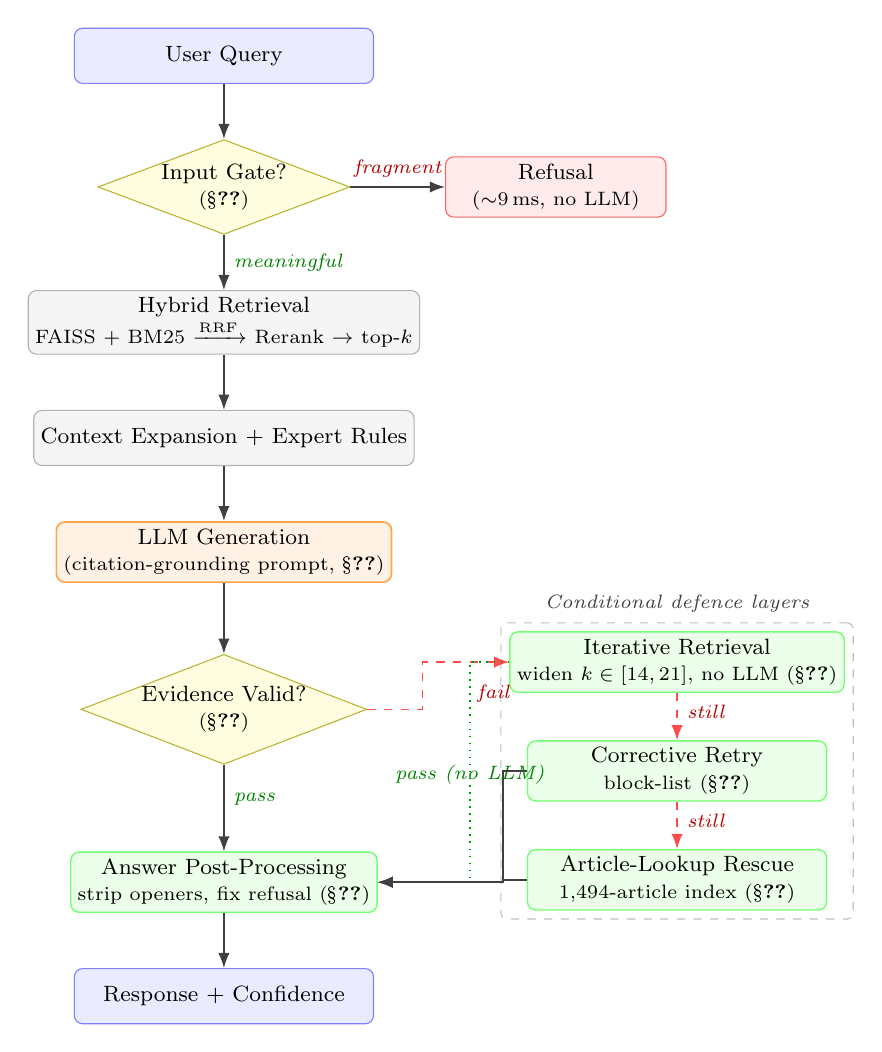
\begin{tikzpicture}[
  >=Latex,
  node distance=7mm and 10mm,
  font=\footnotesize,
  box/.style={draw, rounded corners=3pt, align=center, minimum height=7mm,
              minimum width=38mm, inner sep=2.5pt, line width=0.4pt},
  io/.style={box, fill=blue!8, draw=blue!50},
  stage/.style={box, fill=gray!8, draw=gray!60},
  llm/.style={box, fill=orange!10, draw=orange!70, line width=0.6pt},
  defence/.style={box, fill=green!8, draw=green!55, line width=0.5pt},
  reject/.style={box, fill=red!8, draw=red!60, minimum width=28mm},
  decision/.style={diamond, draw, aspect=2.6, align=center, fill=yellow!12,
                   draw=yellow!70!black, line width=0.4pt, inner sep=0pt,
                   minimum height=8mm, minimum width=32mm},
  flow/.style={->, line width=0.55pt, draw=black!75},
  fail/.style={->, line width=0.55pt, draw=red!70, dashed},
  freeflow/.style={->, line width=0.55pt, draw=green!60!black, dotted},
  passlbl/.style={font=\scriptsize\itshape, text=green!50!black},
  faillbl/.style={font=\scriptsize\itshape, text=red!70!black},
  freelbl/.style={font=\scriptsize\itshape, text=green!50!black},
]
\node[io] (query) {User Query};
\node[decision, below=of query] (gate) {Input Gate?\\\scriptsize (\S\ref{sec:gate})};
\node[reject, right=12mm of gate] (rejected) {Refusal\\\scriptsize ($\sim$9\,ms, no LLM)};
\node[stage, below=of gate] (retrieve) {Hybrid Retrieval\\\scriptsize FAISS + BM25 $\xrightarrow{\mathrm{RRF}}$ Rerank $\to$ top-$k$};
\node[stage, below=of retrieve] (expand) {Context Expansion + Expert Rules};
\node[llm, below=of expand] (gen) {LLM Generation\\\scriptsize (citation-grounding prompt, \S\ref{sec:prompts})};
\node[decision, below=9mm of gen] (validate) {Evidence Valid?\\\scriptsize (\S\ref{sec:validate})};
\node[defence, below=11mm of validate] (postproc) {Answer Post-Processing\\\scriptsize strip openers, fix refusal (\S\ref{sec:postproc})};
\node[io, below=of postproc] (resp) {Response + Confidence};

\node[defence, right=18mm of validate, yshift=6mm] (iter) {Iterative Retrieval\\\scriptsize widen $k\in[14,21]$, no LLM (\S\ref{sec:iter})};
\node[defence, below=6mm of iter] (retry) {Corrective Retry\\\scriptsize block-list (\S\ref{sec:retry})};
\node[defence, below=6mm of retry] (rescue) {Article-Lookup Rescue\\\scriptsize 1{,}494-article index (\S\ref{sec:rescue})};

\draw[flow] (query) -- (gate);
\draw[flow] (gate.east) -- node[faillbl, above, pos=0.5]{fragment} (rejected.west);
\draw[flow] (gate.south) -- node[passlbl, right, pos=0.5]{meaningful} (retrieve.north);
\draw[flow] (retrieve) -- (expand);
\draw[flow] (expand) -- (gen);
\draw[flow] (gen) -- (validate);
\draw[flow] (validate.south) -- node[passlbl, right, pos=0.4]{pass} (postproc.north);
\draw[flow] (postproc) -- (resp);
\draw[fail] (validate.east) -- ++(7mm,0) |- (iter.west);
\node[faillbl] at ($(validate.east)+(16mm,2mm)$) {fail};
\draw[fail] (iter.south) -- node[faillbl, right, pos=0.4]{still} (retry.north);
\draw[fail] (retry.south) -- node[faillbl, right, pos=0.4]{still} (rescue.north);
\draw[freeflow] (iter.west) -- ++(-5mm,0) |- node[freelbl, above, pos=0.3]{pass (no LLM)} (postproc.east);
\draw[flow] (retry.west) -- ++(-3mm,0) |- (postproc.east);
\draw[flow] (rescue.west) -- ++(-3mm,0) |- (postproc.east);
\begin{scope}[on background layer]
  \node[draw=gray!50, dashed, rounded corners=2pt, inner sep=3pt,
        fit=(iter)(retry)(rescue)] (defbox) {};
  \node[anchor=south, font=\scriptsize\itshape, text=gray!50!black]
        at (defbox.north) {Conditional defence layers};
\end{scope}
\end{tikzpicture}
\caption{End-to-end request flow. Solid black arrows = unconditional pipeline;
dashed red = taken on validation failure; dotted green = ``free'' recovery
via iterative retrieval without LLM call. Colour coding:
\textcolor{blue!50}{blue}=I/O, \textcolor{gray!60}{grey}=retrieval,
\textcolor{orange!70}{orange}=LLM, \textcolor{green!55}{green}=defence layers
(contribution of this work).}
\label{fig:pipeline}
\end{figure}

\subsection{Input Gating}\label{sec:gate}

In baseline evaluation, fragmentary user inputs (markdown headings,
single-word bullets such as \ar{* الجناية}, or colon-terminated incomplete
sentences such as \ar{1. ما المقصود بمبدأ:}) frequently triggered the LLM
to \emph{fabricate} a plausible-sounding question and answer it. These cases
accounted for 5 of 28 (17.9\,\%) hallucination instances in baseline
measurements.

A pure function \texttt{is\_meaningful\_query} evaluates the input against a
sequence of regex predicates---minimum Arabic-character count, leading
markdown-header detection, leading list-bullet detection, leading
numbered-fragment detection, trailing-colon check---and short-circuits
failing inputs with a 9-millisecond response. The gate is bypassed when an
uploaded document is present (Section~\ref{sec:upload}). In the v8 evaluation
the gate caught and rejected 8 of 28 inputs without incurring an LLM call.

\subsection{Citation-Grounding Prompts and Law-Naming Disambiguation}\label{sec:prompts}

The prompt-engineering work is itself a substantial contribution and we
document it in detail here. Two distinct prompt-level failure modes were
observed in baseline measurements: (a)~the LLM cites article numbers from
training memory that appear plausible but are not in the retrieved context;
(b)~the LLM confuses substantive (Penal Code) with procedural (Code of
Criminal Procedure) law, citing the wrong code for a given query. For
example, baseline answers to questions about pre-trial detention
(\ar{التوقيف الاحتياطي}) frequently cited Article~300 \emph{of the Penal
Code}---when Article~300 of the Penal Code does not address that topic; the
relevant article is in the Code of Criminal Procedure.

The Conan prompt suite addresses these failure modes with eight rules
explicitly enforced in the system and user prompts:

\begin{enumerate}
  \item \emph{Strict textual adherence}: ``Use the provided texts ONLY''---no
        appeals to general legal principles or international law.
  \item \emph{Citation grounding (absolute)}: ``Cite an article number ONLY
        if those exact digits appear in the Context below.'' If not present,
        write the canonical refusal phrase
        \ar{المادة المطلوبة غير متوفرة في السياق المقدم}.
  \item \emph{Law-naming disambiguation}: procedural matters
        (\ar{التوقيف الاحتياطي، التحقيق، التفتيش، الطعن، النقض}) must be
        cited from \ar{قانون الإجراءات الجنائية}; substantive matters
        (\ar{تعريف الجرائم، أركانها، عقوباتها}) from \ar{قانون العقوبات}.
        Always name the law explicitly when citing.
  \item \emph{Element matching for offence selection}: e.g., for
        injury/assault questions, \ar{المادة 240} requires a permanent
        impairment, \ar{المادة 241} requires $>$\,20 days of incapacity,
        \ar{المادة 242} covers lesser injuries; the prompt explicitly
        instructs the LLM to match the article to the facts rather than
        defaulting to the harshest available.
  \item \emph{Multi-charge handling}: if the case facts describe more than
        one offence (e.g., assault + theft), enumerate the distinct charges
        and analyse each in its own sub-section.
  \item \emph{No casual openings}: explicit prohibition on \ar{حسناً},
        \ar{بالتأكيد}, \ar{تمام}, \ar{طبعاً}, and similar persona-breaking
        fillers; the first word must be part of the answer itself (e.g.,
        \ar{وفقاً للمادة \dots} or \ar{تنص المادة \dots}).
  \item \emph{Incomplete-input handling}: if the user's input is a fragment,
        a heading, a single word, or a sentence ending with a colon, do NOT
        fabricate a question to answer; reply with a polite request for a
        complete question.
  \item \emph{Ambiguity protocol}: if the question is broad (e.g.,
        \ar{ما عقوبة التزوير؟}), provide a brief overview of the cases in
        context and explicitly ask the user to specify the determining
        factors (offender role / document type / weapon / time / injury
        severity) \emph{relevant} to that specific crime---not irrelevant
        factors (e.g., never ask about ``document type'' for a homicide).
\end{enumerate}

In addition, two specialised prompts are used by the defence pipeline:
\texttt{qa\_retry\_ungrounded} for the corrective retry
(Section~\ref{sec:retry}), which receives the original draft and an explicit
list of forbidden article numbers; and \texttt{qa\_rescue\_with\_lookup}
for the article-lookup rescue (Section~\ref{sec:rescue}), which receives
the original retrieved context plus a separate ``Additional References''
block from the article-lookup service and explicitly forbids inventing
neighbouring articles or using a passage about a different law.

\subsection{Evidence Validation}\label{sec:validate}

Every LLM output is post-processed by a regex-based evidence validator. A
canonical extractor (\texttt{extract\_article\_references})---operating on
Arabic-Indic-digit-normalised text---identifies every article number cited
in the answer. The set of cited articles is compared against the set of
article numbers extracted from the retrieved context (concatenated).
Articles cited but not present in the context are flagged as \textbf{missing}
and the answer is marked as failing validation. The same extractor is used
on both sides to avoid spurious mismatches caused by plural-form variations
(\ar{المواد 211، 212، 213} vs \ar{المادة 211}).

\subsection{Corrective Retry with Forbidden-Article Block-List}\label{sec:retry}

When evidence validation flags missing articles, the system re-prompts the
LLM with a correction prompt that includes the original draft and an
\emph{explicit list} of article numbers the LLM must NOT cite. The retry is
run at most \texttt{RETRY\_MAX\_ATTEMPTS} times (default~1---a tuning
informed by the Groq free-tier 6{,}000~tokens-per-minute budget). The
retry's output is accepted only if it strictly improves the missing-article
count.

\subsection{Article-Lookup Rescue}\label{sec:rescue}

Even after retry, a class of hallucinations persisted: the LLM would cite an
article that \emph{did} exist in the dataset, just not in the top-$k$ chunks
for that specific query. Inspection revealed that of 47{,}028 chunks,
14{,}882 (31.6\,\%) carry \texttt{referenced\_articles} metadata covering
1{,}494 distinct article numbers---including, for instance, 34~chunks
referencing Article~87 and 14~chunks referencing Article~300, both articles
the baseline LLM cited ``from memory.''

At startup, \texttt{ArticleLookupService.load()} builds an index
$\{\text{article\_no} \rightarrow [\text{chunk\_index},\ldots]\}$. Chunks
within each article's list are ranked by a three-tier quality score:
\begin{enumerate}
  \item \textbf{Document-type tier}: \texttt{penal\_code} and
        \texttt{criminal\_procedure} (the actual law text) > cassation
        material > encyclopedia / international-law material. This prevents,
        for example, Rome-Statute (ICC) passages from being preferred over
        chunks from the Egyptian code.
  \item \textbf{Article focus}: chunks referencing fewer distinct articles
        are preferred (they are more focused on the queried article).
  \item \textbf{Text length}: longer chunks as a final tiebreaker.
\end{enumerate}

When post-retry evidence validation still flags missing articles, the rescue
path is triggered: the top-2 chunks for each missing article are appended to
the context for one more LLM call. The rescued answer is validated against
the combined context (original + rescue chunks) and accepted only if
grounding improves. The rescue prompt explicitly forbids the LLM from
inventing \emph{neighbouring} articles and from using a passage about a
different law or topic than the user's question.

\subsection{Iterative Retrieval (Adaptive $k$-Expansion)}\label{sec:iter}

Following the spirit of~\cite{alghamdi2023}'s finding that retrieval quality
dominates downstream correctness, we treat $k$ as adaptive. After the initial
generation and validation, if validation flags missing articles AND
\texttt{USE\_ITERATIVE\_RETRIEVAL} is enabled (default), the system re-runs
\emph{only} the retrieval stage---not the LLM---at successively larger $k$
values from \texttt{ITERATIVE\_K\_SEQUENCE} (default $[7,14,21]$). Any new
chunks not already in the context are appended; if any widened window
surfaces the missing articles, validation passes \emph{for free}. Only if
this cheap expansion still fails does the corrective retry
(Section~\ref{sec:retry}) and rescue (Section~\ref{sec:rescue}) take over,
but now with a wider context in hand. Easy queries pay no extra cost; hard
queries pay 2--3 cheap retrievals before an LLM call is incurred.

\subsection{Answer Post-Processing}\label{sec:postproc}

A deterministic, regex-driven post-processing layer
(\texttt{postprocess\_answer}) runs after the final answer is selected.
Two transformations:
\begin{enumerate}
  \item \emph{Casual-opener stripping}---a curated list of conversational
        fillers (\ar{حسناً}, \ar{بالتأكيد}, \ar{تمام}, \ar{طبعاً},
        \ar{سوف أجيب}, \ar{لقد قرأت السؤال}, \ldots) is stripped from the
        leading position; multi-word openers ordered longest-first to
        prevent stranded fragments.
  \item \emph{Refusal-phrase normalisation}---when the LLM splices the
        template-refusal phrase \ar{المادة المطلوبة غير متوفرة في السياق
        المقدم} mid-clause, the regex \texttt{\_EMBEDDED\_REFUSAL\_RE}
        matches the awkward construction---accounting for Arabic
        prefix-contraction (\ar{ل + ال} $\rightarrow$ \ar{لل})---and rewrites
        it as a standalone sentence.
\end{enumerate}

\subsection{Procedural-Defence Reasoning Checklist for Case Analysis}\label{sec:checklist}

The grounding mechanisms above ensure that what the system \emph{cites} is
correct; a complementary failure mode concerns what it \emph{omits}. The
case-analysis endpoints (\texttt{/weakness}, \texttt{/defense},
\texttt{/forensic}) take a full criminal case file rather than a single
question, and a domain expert's review of their output scored the legal
reasoning at roughly 70\,\%: the analyses were well-grounded but missed
several high-value procedural-nullity and criminal-intent arguments that a
practising Egyptian criminal-defence lawyer applies routinely, and in one
instance over-claimed a defect that did not exist. We encode the expert's
feedback as a \textbf{procedural-defence checklist} of five reasoning
procedures appended to the system prompts of the three case-analysis
endpoints and reinforced in their user templates:

\begin{enumerate}
  \item[\textbf{A.}] \emph{Timeline vs.\ prosecution warrant}---compare the
        exact time of the arrest/search against the time the prosecution
        warrant (\ar{إذن النيابة}) issued; a seizure preceding the warrant
        voids the arrest and everything built on it
        (\ar{ما بُني على باطل فهو باطل}). The rule explicitly instructs the
        model to read \ar{الساعة 12:00 صباحاً} as the \emph{start} of the day,
        correcting a clock-reading error observed in baseline output.
  \item[\textbf{B.}] \emph{Identifier mismatch}---compare every identifier in
        the warrant (vehicle plate numbers, names, IDs) against the seizure
        record; any discrepancy places the seized item outside the warrant
        and may evidence \ar{تلفيق}.
  \item[\textbf{C.}] \emph{Territorial jurisdiction}---apply correctly and do
        \emph{not} over-claim spatial excess for a location inside the
        precinct; this point is a precision correction (a false-positive
        suppressor) rather than an additional-recall rule.
  \item[\textbf{D.}] \emph{Chain of custody}---challenge the integrity of the
        sealed exhibits (\ar{التحريز}) when the officer who sealed them
        differs from the one who wrote the seizure record.
  \item[\textbf{E.}] \emph{Intent from profession}---weigh the defendant's
        occupation against the nature of any seized cash to contest
        trafficking intent (\ar{انتفاء قصد الاتجار}).
\end{enumerate}

The checklist is paired with a single fully-worked, \emph{fictional} few-shot
exemplar demonstrating all five points end-to-end. Crucially, the exemplar is
\textbf{grounding-safe by construction}: it names defence doctrines
(\ar{بطلان القبض والتفتيش}, \ar{انتفاء قصد الاتجار}) but contains
\emph{no} \ar{المادة}~$N$ article number, so it cannot teach the model to
emit an ungrounded citation that the evidence validator
(Section~\ref{sec:validate}) would flag---raising reasoning coverage while
preserving the 0\,\% hallucinated-citation property. Each checklist item is
explicitly conditioned on the facts supporting it (``raise a point only when
the facts genuinely support it---never invent one''), so the additions
trade no precision for their gain in recall.

A companion \textbf{charge-fidelity} rule extends the same precision
principle to the offences themselves: the case-analysis endpoints are
constrained to enumerate only offences actually charged or described in the
case file, and are explicitly forbidden from inventing an uncharged offence
(e.g., adding \ar{قيادة بدون رخصة} when the file never mentions a licence).
This closes a fabrication mode observed during live validation, where the
generator appended a plausible-but-uncharged offence to an otherwise
grounded analysis.

The agentic self-check that closes the argument-level (not merely
citation-level) hallucination gap for defence memoranda is described as part of
the multi-agent pipeline in Section~\ref{sec:selfcheck}, and the full agentic
case-analysis flow these case-analysis endpoints invoke is the subject of
Section~\ref{sec:agentic}.

% =============================================================================
\section{Multi-Agent Agentic Case-Analysis Pipeline}\label{sec:agentic}

Single-question Q\&A is well served by the layered defence pipeline of
Section~\ref{sec:defence}. \emph{Open-ended case work}---reading a full criminal
case file and producing a weakness analysis or a defence memorandum---is a
qualitatively harder task: it requires extracting structured facts, hypothesising
multiple independent lines of defence, grounding each one in its own statutory and
precedential authority, judging which arguments actually hold, and only then
writing. A single-shot ``case\,$\rightarrow$\,LLM\,$\rightarrow$\,output'' prompt
collapses all of these into one undifferentiated generation, where the model
reasons over everything at once from a single retrieval and tends both to miss
high-value arguments and to assert claims it cannot support. We therefore replace
the single-shot path for \texttt{/weakness} and \texttt{/defense} with an
\textbf{agentic, multi-agent pipeline} (\texttt{USE\_AGENTIC\_PIPELINE}, on by
default) that decomposes the task into six specialised agents with a deterministic
orchestrator. Figure~\ref{fig:agentic} shows the flow; Table~\ref{tab:agents}
details each agent.

\begin{figure}[!t]
\centering
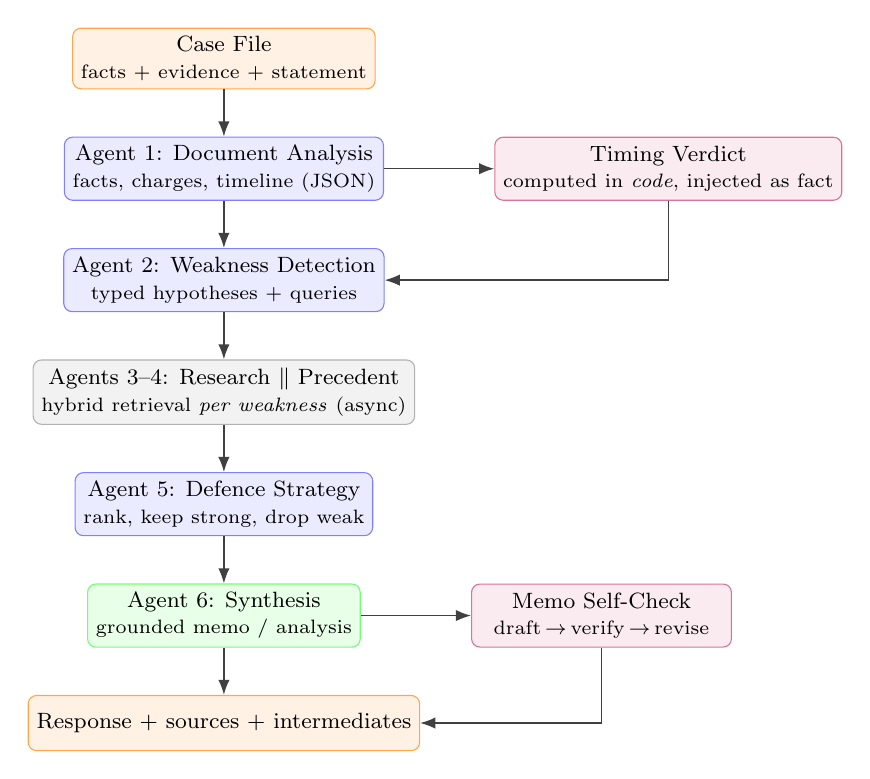
\begin{tikzpicture}[
  >=Latex, font=\footnotesize, node distance=6mm and 9mm,
  ag/.style={draw, rounded corners=3pt, align=center, minimum height=8mm,
             minimum width=33mm, inner sep=3pt, fill=blue!8, draw=blue!50,
             line width=0.4pt},
  sym/.style={draw, rounded corners=3pt, align=center, minimum height=8mm,
              minimum width=33mm, inner sep=3pt, fill=purple!8, draw=purple!55},
  ret/.style={draw, rounded corners=3pt, align=center, minimum height=8mm,
              minimum width=33mm, inner sep=3pt, fill=gray!10, draw=gray!60},
  outp/.style={draw, rounded corners=3pt, align=center, minimum height=8mm,
              minimum width=33mm, inner sep=3pt, fill=green!9, draw=green!55},
  io/.style={draw, rounded corners=3pt, align=center, minimum height=7mm,
             minimum width=26mm, inner sep=3pt, fill=orange!10, draw=orange!70},
  fl/.style={->, line width=0.55pt, draw=black!75},
]
\node[io] (case) {Case File\\\scriptsize facts + evidence + statement};
\node[ag, below=of case] (a1) {Agent 1: Document Analysis\\\scriptsize facts, charges, timeline (JSON)};
\node[sym, right=14mm of a1] (sym) {Timing Verdict\\\scriptsize computed in \emph{code}, injected as fact};
\node[ag, below=of a1] (a2) {Agent 2: Weakness Detection\\\scriptsize typed hypotheses + queries};
\node[ret, below=of a2] (a34) {Agents 3--4: Research $\|$ Precedent\\\scriptsize hybrid retrieval \emph{per weakness} (async)};
\node[ag, below=of a34] (a5) {Agent 5: Defence Strategy\\\scriptsize rank, keep strong, drop weak};
\node[outp, below=of a5] (a6) {Agent 6: Synthesis\\\scriptsize grounded memo / analysis};
\node[sym, right=14mm of a6] (sc) {Memo Self-Check\\\scriptsize draft\,$\to$\,verify\,$\to$\,revise};
\node[io, below=of a6] (resp) {Response + sources + intermediates};

\draw[fl] (case) -- (a1);
\draw[fl] (a1) -- (a2);
\draw[fl] (a1.east) -- (sym.west);
\draw[fl] (sym.south) |- (a2.east);
\draw[fl] (a2) -- (a34);
\draw[fl] (a34) -- (a5);
\draw[fl] (a5) -- (a6);
\draw[fl] (a6.east) -- (sc.west);
\draw[fl] (sc.south) |- (resp.east);
\draw[fl] (a6) -- (resp);
\end{tikzpicture}
\caption{The six-agent case-analysis pipeline. Blue = LLM agents emitting
checkable JSON; grey = hybrid retrieval grounding each weakness in its own
authority; purple = \emph{neuro-symbolic} components (a code-computed timing
verdict injected as a hard fact, and the draft\,$\rightarrow$\,verify\,$\rightarrow$\,revise
self-check); green = grounded synthesis. On any critical-agent failure the
orchestrator raises \texttt{AgentPipelineError} and the router falls back to the
single-shot path.}
\label{fig:agentic}
\end{figure}

\subsection{Agents and orchestration}

\begin{table*}[!htb]
\centering
\small
\caption{Roles of the six agents in the case-analysis pipeline. Intermediate
agents are forced to emit strict JSON (robustly parsed with a balanced-brace
fallback), so each stage's output is machine-checkable before the next consumes
it.}
\label{tab:agents}
\setlength{\tabcolsep}{5pt}
\renewcommand{\arraystretch}{1.25}
\begin{tabular}{L{1.0cm} L{3.1cm} L{6.0cm} L{3.6cm}}
\toprule
\rowcolor{tabhead}
\thead{\#} & \thead{Agent} & \thead{Function} & \thead{Output} \\
\midrule
1 & Document Analysis & Extract structured facts, parties, charges, evidence items, and a dated/timed chronological timeline from the case file & JSON: facts, charges, \texttt{timeline} \\
\rowcolor{tabalt}
2 & Weakness Detection & Turn the analysis into typed weakness hypotheses, each with a focused legal-research query & JSON list of weaknesses \\
3--4 & Legal Research \& Precedent Retrieval & For each top weakness, one hybrid retrieval whose pool yields both doctrine/statute and court-precedent chunks (split by \texttt{doc\_type}); run concurrently & Contexts + sources per weakness \\
\rowcolor{tabalt}
5 & Defence Strategy & Rank weaknesses against the \emph{retrieved} authorities, keep the strong, discard the disproven, order the argument & JSON: kept + ordered IDs \\
6 & Synthesis & Write the final Arabic weakness analysis or four-part defence memorandum from the kept, grounded authorities only & Arabic text + sources \\
\bottomrule
\end{tabular}
\end{table*}

The orchestrators \texttt{run\_weakness\_pipeline} and
\texttt{run\_defense\_pipeline} share one private \texttt{\_run\_pipeline}. After
Agent~2, only the top \texttt{AGENT\_MAX\_WEAKNESSES} ($=6$) weaknesses are
researched in depth; the rest are carried with their hypothesis text. The
per-weakness retrievals (Agents~3--4) are launched concurrently with
\texttt{asyncio.gather}, but the actual CPU concurrency is bounded by the reranker
semaphore, so a full memo stays CPU-affordable on the laptop deployment ($\sim$2--3
minutes rather than $\sim$10). A single weakness failing to retrieve does not sink
the run (\texttt{return\_exceptions=True} filters it out); only if \emph{every}
weakness fails, or a critical agent (analysis, detection, strategy, synthesis)
errors, does the orchestrator raise \texttt{AgentPipelineError}---at which point the
router silently falls back to the single-shot path. The pipeline is thus never a
hard dependency. The orchestrator also returns the structured intermediates
(timeline, weaknesses, authorities, sources) alongside the final text, so the
client can render the reasoning trace, not just the conclusion.

\subsection{Neuro-symbolic grounding: the deterministic timing verdict}\label{sec:timing}

The single most damaging recurring error in case analysis was \emph{chronological}:
the model repeatedly mis-read whether the arrest/search happened before or after
the prosecution warrant (\ar{إذن النيابة})---inverting the order even when the
timeline was extracted correctly---and a wrong verdict here flips the entire
defence. Rather than prompt harder, we move this judgement out of the LLM
entirely. \texttt{compute\_timing\_verdict} parses each timeline event's Arabic
date and time string (handling \ar{صباحاً}/\ar{مساءً}/\ar{منتصف الليل} and the
\ar{الساعة 12:00 صباحاً}-as-midnight convention), computes the signed gap between
warrant and seizure in code, and emits one of three deterministic verdicts: seizure
\emph{before} the warrant (the nullity argument \ar{بطلان القبض والتفتيش} applies,
with \ar{ما بُني على باطل فهو باطل}), \emph{within} the 24-hour validity window (the
timing is sound and the ``arrest preceded the warrant'' plea is \emph{forbidden} as
contrary to the record), or \emph{after} the window expired (a different nullity
applies). This verdict is injected into the downstream agents' context as a hard
fact they cannot re-derive incorrectly---a small but decisive neuro-symbolic
component that converts a stubborn reasoning failure into a solved sub-problem.

\subsection{Argument-level self-check}\label{sec:selfcheck}

Per-answer evidence validation (Section~\ref{sec:validate}) catches fabricated
article \emph{numbers}, but a memorandum can also contain fabricated
\emph{reasoning}---an assertion the case facts do not support, or an argument with
no authority behind it. The defence-memorandum endpoint therefore applies an
additional \textbf{agentic self-check} (\texttt{MEMO\_SELF\_CHECK}): the draft is
fed back to the LLM under a dedicated reviewer prompt (\texttt{verify\_memo}) whose
sole instruction is to make the memo \emph{fully grounded} in the provided
material---removing or correcting any article number not present in the retrieved
texts, deleting any assertion the facts do not support, and introducing no new
citation or fact---while preserving the four-part structure (\ar{الوقائع},
\ar{الإطار القانوني}, \ar{أوجه الدفاع}, \ar{الطلبات}). The
draft\,$\rightarrow$\,verify\,$\rightarrow$\,revise loop runs up to
\texttt{MEMO\_SELF\_CHECK\_MAX\_ITERS} times (default~1), stops early once a pass
both validates and introduces no further change, and never raises---on any LLM
failure it returns the best text so far. The number of revision passes applied is
surfaced to the client as \texttt{self\_check\_revisions}.

% =============================================================================
\section{Document Upload Pipeline}\label{sec:upload}

The system supports three retention semantics for user-supplied documents,
all flowing through a single shared parser (\texttt{services/upload\_helper.py})
to guarantee consistent behaviour:
\begin{itemize}
  \item \texttt{POST /api/v1/qa/upload}---per-question attachment (not
        persisted);
  \item \texttt{POST /api/v1/chat/attach}---session-attached document
        (persists with the chat session on disk);
  \item \texttt{POST /api/v1/ingest}---permanent corpus ingestion (merges
        into FAISS and BM25, hot-reloaded by the running service).
\end{itemize}

Supported formats: \texttt{.txt} (with Arabic-encoding fallback), \texttt{.pdf}
(\texttt{pdftotext} preferred, PyPDF2 fallback), and \texttt{.docx}
(\texttt{docx2txt}). The legacy \texttt{.doc} binary format is explicitly
rejected with a helpful Arabic message recommending conversion to
\texttt{.docx} or \texttt{.pdf}.

\paragraph{Automated ingestion and hot-reload} Permanent ingestion is also
available without a manual API call. A watch-folder daemon
(\texttt{watch\_ingest.py}) polls an inbox directory
(\texttt{INGEST\_INBOX\_DIR}) every \texttt{INGEST\_WATCH\_INTERVAL\_S} seconds
(default 30) and ingests any new files through the same parser and
Arabic-cleaning path as the manual pipeline, tracking already-processed paths
in \texttt{data/.ingested\_files.json} so the operation is idempotent. The
same scan is exposed as \texttt{POST /api/v1/ingest/scan}, which runs the scan
in a worker thread and then calls \texttt{reload\_indices()} to hot-swap the
FAISS, BM25, chunk, and tokenised-corpus state of the running service
\emph{in place}---without re-initialising the embedding model or restarting
the process. The four index files are always written and reloaded together to
keep retrieval state coherent.

% =============================================================================
\section{Evaluation}\label{sec:eval}

\subsection{Benchmark}\label{sec:baseline}

We constructed a 28-question Arabic legal benchmark spanning three difficulty
tiers (basics, application, advanced) and covering both substantive (Penal
Code) and procedural (Code of Criminal Procedure) law. The benchmark
deliberately includes 5 well-formed substantive questions, 1 procedural
question that historically triggered wrong-law confusion, 5 input-gate test
cases (markdown headings, bullets, colon-terminated incomplete sentences),
and 17 application and reasoning questions drawn from undergraduate
criminal-law curricula. Each question is evaluated against two metrics:
(i)~\emph{evidence-validation status}---whether every article number cited in
the answer can be traced to the retrieved (or rescued) context---and
(ii)~the \emph{confidence score} of Equation~\ref{eq:conf}.

\subsection{Results across system versions}

Table~\ref{tab:results} summarises headline metrics across five system
versions corresponding to the cumulative introduction of each
grounding-defence layer.

\begin{table}[!htb]
\centering
\small
\caption{Headline metrics across five system versions on the 28-question
benchmark. v5 (multi-query expansion) is omitted: see
Section~\ref{sec:limits}. Mean API latency excludes input-gated rows (which
do not invoke an LLM and complete in $\sim$9\,ms). The v8 LLM upgrade
(llama-3.1-8b $\rightarrow$ llama-3.3-70b) is also responsible for the
substantial mean-latency reduction, since the larger model triggers fewer
corrective retries.}
\label{tab:results}
\setlength{\tabcolsep}{4pt}
\renewcommand{\arraystretch}{1.15}
\begin{tabular}{lrrrrr}
\toprule
\rowcolor{tabhead}
\thead{Metric}               & \thead{v3} & \thead{v4} & \thead{v6} & \thead{v7} & \thead{v8} \\
\midrule
Passed validation            &  20/28 &  26/28 &  27/28 &  27/28 & \textbf{28/28} \\
\quad (\%)                   & 71.4\% & 92.9\% & 96.4\% & 96.4\% & \textbf{100.0\%} \\
Hallucinations               &   8/28 &   2/28 &   1/28 &   1/28 & \textbf{0/28}  \\
\quad (\%)                   & 28.6\% &  7.1\% &  3.6\% &  3.6\% & \textbf{0.0\%} \\
Avg confidence               & 41.2\% & 38.0\% & 39.8\% & 40.0\% & 41.9\% \\
Input-gated (no LLM)         &      0 &      8 &      8 &      8 &      8 \\
\midrule
Mean API latency (ms)        & 26{,}028 & 34{,}162 & 34{,}096 & 33{,}459 & \textbf{18{,}390} \\
Max API latency (ms)         & 48{,}691 & 64{,}439 & 116{,}940 & 107{,}427 & 28{,}460 \\
Mean retrieval latency (ms)  & 13{,}479 & 17{,}193 & 16{,}508 & 13{,}587 & 16{,}024 \\
\bottomrule
\end{tabular}
\end{table}

Progression by layer:
\begin{itemize}
  \item v3 $\rightarrow$ v4: input gate + corrective retry + tightened
        prompts $\rightarrow -21.5$ pp (8 $\rightarrow$ 2).
  \item v4 $\rightarrow$ v6: article-lookup rescue $\rightarrow -3.5$ pp
        (2 $\rightarrow$ 1).
  \item v6 $\rightarrow$ v7: rescue prompt tightening + quality-tiered chunk
        ranking $\rightarrow$ 0 net change in pass rate, but the failing
        question shifted (LLM non-determinism).
  \item v7 $\rightarrow$ v8: LLM upgrade from
        \texttt{llama-3.1-8b-instant} to \texttt{llama-3.3-70b-versatile}
        $\rightarrow -3.6$ pp (1 $\rightarrow$ 0).
\end{itemize}

\subsection{Per-category breakdown}

Table~\ref{tab:bycat} disaggregates the headline pass-rate by question
category, exposing which defence layers recover which failure modes. The
benchmark's 28 questions break down into 11~substantive (definitions of
crimes, penalties, elements), 1~procedural (pre-trial detention),
8~fragment / input-gate tests (markdown headers, bullets, colon-terminated
sentences), and 8~reasoning / application questions (case analyses,
comparisons, hypotheticals).

\begin{table}[!htb]
\centering
\small
\caption{Pass rate by question category across versions. Substantive
questions absorb the largest share of the v3 baseline failures (3/11); these
are recovered progressively by the corrective retry (v4), the article-lookup
rescue (v6), and the LLM upgrade (v8). Fragment failures in v3 reflect
hallucinated answers to inputs the system should have refused; they are
fully resolved by the input gate introduced in v4.}
\label{tab:bycat}
\setlength{\tabcolsep}{5pt}
\renewcommand{\arraystretch}{1.15}
\begin{tabular}{lcccccr}
\toprule
\rowcolor{tabhead}
\thead{Category} & \thead{v3} & \thead{v4} & \thead{v6} & \thead{v7} & \thead{v8} & \thead{total} \\
\midrule
Substantive    & 8/11  & 9/11  & 10/11  & 10/11  & \textbf{11/11} & 11 \\
Procedural     & 0/1   & 1/1   & 1/1    & 1/1    & \textbf{1/1}   & 1  \\
Reasoning      & 7/8   & 8/8   & 8/8    & 8/8    & \textbf{8/8}   & 8  \\
Fragment       & 5/8   & 8/8   & 8/8    & 8/8    & \textbf{8/8}   & 8  \\
\midrule
\textbf{Total} & 20/28 & 26/28 & 27/28  & 27/28  & \textbf{28/28} & 28 \\
\bottomrule
\end{tabular}
\end{table}

\subsection{Per-question transition for historically-failing rows}

Table~\ref{tab:transition} traces the nine questions that failed
evidence-validation in at least one version. The cell format \emph{S~XX\%}
encodes status (\emph{P}=pass / \emph{F}=fail) and confidence percentage.
Several observations are noteworthy:

\begin{itemize}
  \item \textbf{Q2} (the most persistent substantive failure --- legitimate
        self-defence, hallucinating \protect\ar{المادة 87}) failed in v3
        through v6 and was only resolved by the v7 article-lookup-rescue
        prompt tightening + better chunk ranking. v8 retains the fix.
  \item \textbf{Q18} (\protect\ar{الجريمة تامة أم شروع}) is the system's
        non-deterministic worst-case. The LLM cites a different fabricated
        article number on each run (Articles 30, 31, 32 observed). The
        article-lookup rescue catches whichever number it cites when that
        number exists in the index --- which is why v6 and v8 pass but v7
        (with a regression of the rescue prompt) failed.
  \item \textbf{Fragment rows} (Q6, Q13, Q23) all pass from v4 onward with
        0\,\% confidence by design --- the input gate short-circuits them
        before any LLM call.
\end{itemize}

\begin{table}[!htb]
\centering
\small
\caption{Per-version status and confidence for the 9 questions that failed
in at least one version. P = passed evidence validation; F = failed
(hallucinated citation). The other 19 questions pass in every version and
are omitted for brevity. Confidence is rounded to the nearest percent.}
\label{tab:transition}
\setlength{\tabcolsep}{3.5pt}
\renewcommand{\arraystretch}{1.18}
\begin{tabular}{rllllllp{4.8cm}}
\toprule
\rowcolor{tabhead}
\thead{\#} & \thead{cat} & \thead{v3} & \thead{v4} & \thead{v6} & \thead{v7} & \thead{v8} & \thead{Question (truncated)} \\
\midrule
 2 & sub.  & F\,12\% & F\,2\%  & F\,2\%  & P\,57\% & P\,62\% & \ar{الدفاع الشرعي في قانون العقوبات} \\
 3 & proc. & F\,9\%  & P\,59\% & P\,59\% & P\,59\% & P\,55\% & \ar{شروط التوقيف الاحتياطي} \\
 4 & sub.  & F\,20\% & P\,70\% & P\,70\% & P\,70\% & P\,70\% & \ar{أركان جريمة القتل العمد} \\
 6 & frag. & F\,0\%  & P\,0\%  & P\,0\%  & P\,0\%  & P\,0\%  & \ar{\#\# المستوى الأول --- أساسيات} \\
13 & frag. & F\,0\%  & P\,0\%  & P\,0\%  & P\,0\%  & P\,0\%  & \ar{* المخالفة} \\
18 & sub.  & P\,53\% & F\,0\%  & P\,48\% & F\,0\%  & P\,53\% & \ar{هل تعتبر الجريمة تامة أم شروع؟} \\
23 & frag. & F\,0\%  & P\,0\%  & P\,0\%  & P\,0\%  & P\,0\%  & \ar{\#\# المستوى الثالث} \\
25 & sub.  & F\,14\% & P\,64\% & P\,64\% & P\,64\% & P\,64\% & \ar{الفاعل الأصلي والشريك في الجريمة} \\
28 & reas. & F\,0\%  & P\,47\% & P\,47\% & P\,47\% & P\,47\% & \ar{أسباب الإباحة وموانع المسؤولية} \\
\bottomrule
\end{tabular}
\end{table}

\subsection{Comparison with related work}

Direct numerical comparison with prior Arabic-legal-RAG work is complicated
by the fact that no two papers in the area share a common benchmark---each
publishes against its own custom dataset. Table~\ref{tab:compare} reports
each system's headline metric on its own evaluation, alongside the
qualitative comparisons that \emph{are} comparable.

\begin{table}[!htb]
\centering
\caption{Comparison with related Arabic-legal-RAG work. Metric column reports
each paper's primary reported figure on its own benchmark.}
\label{tab:compare}
\setlength{\tabcolsep}{3pt}
\renewcommand{\arraystretch}{1.20}
\begin{tabular}{lllr}
\toprule
\rowcolor{tabhead}
\thead{System} & \thead{Domain} & \thead{Primary metric} & \thead{Score} \\
\midrule
El-Beltagy \& Abdallah~\cite{elbeltagy2024}
       & Arabic RAG (general)
       & embedding-model ablations
       & --- \\
Hrimech et~al.~\cite{hrimech2025}
       & Moroccan family code
       & MRR, Recall@$k$, F1
       & --- \\
Aboasal et~al.~\cite{aboasal2025}
       & Egyptian legal IR
       & MAP / nDCG@10
       & 0.83 / 0.86 \\
Abu Shairah et~al.~\cite{alarb2025}
       & Saudi commercial law
       & verdict prediction
       & --- \\
\midrule
\textbf{Conan (this work)}
       & \textbf{Egyptian criminal law}
       & \textbf{hallucination rate}
       & \textbf{0.0\%} \\
\textbf{Conan (this work)}
       & \textbf{Egyptian criminal law}
       & \textbf{validation pass rate}
       & \textbf{100\%} \\
\bottomrule
\end{tabular}
\end{table}

Beyond headline metrics, Table~\ref{tab:features} contrasts \emph{capabilities}.
The cited prior work concentrates on the retrieval stage; none reports a
post-generation grounding-defence pipeline, an agentic case-analysis flow, or an
open Egyptian-criminal-law corpus.

\begin{table*}[!htb]
\centering
\small
\caption{Capability comparison with related Arabic-legal-RAG work.
\YES~present, \NO~not reported. ``Hybrid'' = dense + sparse retrieval.}
\label{tab:features}
\setlength{\tabcolsep}{4pt}
\renewcommand{\arraystretch}{1.25}
\begin{tabular}{L{4.3cm} C{1.7cm} C{1.7cm} C{1.7cm} C{1.7cm} C{1.9cm}}
\toprule
\rowcolor{tabhead}
\thead{Capability} & \thead{El-Beltagy~\cite{elbeltagy2024}} & \thead{Hrimech~\cite{hrimech2025}} & \thead{Aboasal~\cite{aboasal2025}} & \thead{ALARB~\cite{alarb2025}} & \thead{Conan} \\
\midrule
Hybrid retrieval (dense+sparse) & \NO & \NO & \YES & \NO & \YES \\
\rowcolor{tabalt}
Cross-encoder reranking & \NO & \NO & \NO & \NO & \YES \\
Post-gen.\ hallucination defence & \NO & \NO & \NO & \NO & \YES \\
\rowcolor{tabalt}
Evidence/citation validation & \NO & \NO & \NO & \NO & \YES \\
Agentic multi-agent pipeline & \NO & \NO & \NO & \NO & \YES \\
\rowcolor{tabalt}
Neuro-symbolic reasoning tool & \NO & \NO & \NO & \NO & \YES \\
Both substantive + procedural law & \NO & \NO & \NO & \NO & \YES \\
\rowcolor{tabalt}
Document upload / ingestion & \NO & \NO & \NO & \NO & \YES \\
Production service + wire contract & \NO & \NO & \NO & \NO & \YES \\
\rowcolor{tabalt}
Open released corpus & \NO & \NO & \NO & \YES & \YES \\
\bottomrule
\end{tabular}
\end{table*}

Our chosen primary metric (hallucination rate) differs from the
information-retrieval metrics used by~\cite{aboasal2025} and~\cite{hrimech2025}
deliberately. As Hrimech et~al.~\cite{hrimech2025} explicitly observe,
``content validity of legal clauses reproduced from retrieval systems'' is
the practical bottleneck in deploying these systems to legal practice---and
that is what our hallucination-rate metric measures directly. Three
distinguishing properties of our setup are worth highlighting:
\begin{itemize}
  \item \emph{Wider scope of source material}: 1{,}057 documents and 47{,}028
        chunks vs. 500 articles / 1{,}000 Q\&A in~\cite{aboasal2025} and
        2{,}500 Q\&A pairs in~\cite{hrimech2025}.
  \item \emph{Coverage of both substantive and procedural law} (Penal Code +
        Code of Criminal Procedure), with explicit prompt-level disambiguation.
        Prior Arabic-legal-RAG work tends to focus on one or the other.
  \item \emph{Layered post-generation defence pipeline} not present in any of
        the cited prior work, which focus exclusively on the retrieval stage.
\end{itemize}

\subsection{Cross-model benchmark (protocol)}\label{sec:crossmodel}

To situate Conan against general-purpose frontier models on Arabic legal
questions, we provide a head-to-head harness (\texttt{benchmark\_llms.py})
that queries our full RAG system alongside \texttt{openai/gpt-4o-mini} and
\texttt{anthropic/claude-sonnet-4.5} (both routed through a single OpenRouter
key for cost parity). It runs in two modes that isolate two distinct
questions:
\begin{itemize}
  \item \emph{RAG mode} --- all three models answer from the \emph{same}
        retrieved context, isolating answer-synthesis quality from retrieval;
  \item \emph{Raw mode} --- each model answers from its own parametric
        knowledge with no retrieval, probing baseline Arabic
        criminal-law knowledge.
\end{itemize}
Each run emits a per-model CSV recording latency, answer length, and the set
of cited article numbers, against which the same evidence-validation extractor
(Section~\ref{sec:validate}) is applied to measure citation grounding on equal
footing. \emph{Quantitative results are pending a full benchmark run and will
be reported in a subsequent revision;} at the time of writing the comparison
could not be executed because of API-access limits on the shared OpenRouter
key. The protocol is documented here so the comparison is reproducible once
access is restored.

\subsection{Qualitative observations}

Two questions are particularly informative. \textbf{Q3}
(\ar{التوقيف الاحتياطي}): in v3, this triggered the wrong-law failure mode
(cited Article~300 of the Penal Code); after prompt-level disambiguation in
v4, the LLM correctly identifies the question as procedural and produces a
refusal-style answer when retrieval does not surface the relevant chunks.
Validation passes (no fabricated citation) at 59\,\% confidence.
\textbf{Q18} (\ar{هل تعتبر الجريمة تامة أم شروع؟}) was the most persistent
failure: it failed in v3, regressed under v4's pure-prompt approach (citing
Articles~30 and~31), and recovered to passing only with the article-lookup
rescue in v6 (\ar{تم استرجاع مواد إضافية من قاعدة البيانات للتحقق من
الاستشهادات (مواد: 30, 31)}), at 48\,\% confidence. These cases underline
that no single mechanism is sufficient: each layer recovers a distinct
class of failure.

\subsection{Retrieval-quality optimisation (v9): embeddings, chunking,
reranking, and a scored harness}\label{sec:retropt}

The v3$\to$v8 evolution (Table~\ref{tab:results}) drove \emph{citation
fidelity}---what the system cites, given its context---to a 0\,\% hallucination
rate. It did not address the complementary ceiling: whether the authoritative
article ever \emph{reaches} the context. A grounding pipeline can only validate
citations against what retrieval surfaces; if the relevant article never enters
the top-$k$, the best achievable outcome is an honest refusal, not a correct
answer. The v9 work targets retrieval quality directly, along four axes, and
introduces the measurement instrument that makes such tuning auditable.

\paragraph{Motivation: the retrieval ceiling} Three structural weaknesses
bounded recall. (i)~The embedder was \texttt{paraphrase-multilingual-MiniLM-L12-v2}
(384-dim), a general-purpose multilingual encoder chosen for fast CPU rebuilds;
it is not domain-tuned, is comparatively weak on Arabic legal phrasing, and its
512-token cap silently truncated longer statute chunks. (ii)~Chunking was purely
character-recursive, so a single article's text could be split across a boundary
or share a chunk with an unrelated neighbour, diluting the signal for the exact
unit a citation-driven system must retrieve. (iii)~The cross-encoder reranker
re-scored only the top-10 RRF candidates, so a relevant chunk fused at rank~11 or
lower could never be promoted.

\paragraph{Enhancement~1: embedding upgrade (MiniLM-384 $\to$ BGE-M3-1024)} We
integrate \texttt{BAAI/bge-m3} (1{,}024-dim) behind the embedding configuration as
the target encoder: a multilingual model with strong Arabic retrieval and native
long-context support (sequence length raised $512\to1{,}024$, eliminating
truncation), consistent with Aboasal~et~al.~\cite{aboasal2025} reporting
substantially higher MAP with BGE-M3 on a comparable Arabic legal task. As
dimensionality changes, deploying it requires a full FAISS rebuild, performed into
a staging directory and swapped atomically so the live index keeps serving. The
rollout is deferred (see \emph{Deployment status} below) but the path is fully
prepared.

\paragraph{Enhancement~2: article-aware chunking} For statute-structured document
types (Penal Code, Code of Criminal Procedure, legal-reference collections) the
chunker splits on article-header boundaries (\ar{المادة N}), emitting each article
as a single intact chunk; only an article exceeding the doc-type chunk size is
sub-split, and narrative material (cases, rulings, encyclopedia) keeps recursive
character splitting. Each article-anchored chunk carries a new
\texttt{primary\_article} field---the article the chunk \emph{is}, rather than one
it merely cross-references---preferred when populating the per-source article field
and feeding the article-validation and topic-match confidence signals. The chunker
is the single source of truth shared by the batch builder and the incremental
ingest pipeline, so the two index-writers cannot drift.

\paragraph{Enhancement~3: wider reranker pool} The cross-encoder now re-scores the
top-50 RRF candidates rather than the top-10, rescuing relevant chunks fused at low
rank. The cost is a modest per-query CPU increase and no rebuild---the one
zero-cost, immediately-deployable lever of the four.

\paragraph{Enhancement~4: a scored evaluation harness} To make retrieval tuning
measurable rather than impressionistic, \texttt{eval\_harness.py} scores a labeled
gold set and emits a machine-readable scorecard. A \emph{retrieval mode} (LLM-free)
measures the ceiling---recall@k, article-recall, primary-hit@k (whether a retrieved
chunk \emph{is} an expected article, a direct test of article-aware chunking), and
MRR; an \emph{end-to-end mode} scores citation recall, hallucination rate,
out-of-scope abstention, confidence calibration, and latency against the live API.
A \texttt{--compare} mode diffs two scorecards. This harness is the backbone for
the before/after comparison once the embedding rollout lands, and for all future
tuning.

\paragraph{Deployment status and the CPU-embedding constraint} The four
enhancements differ in deployment cost. The widened reranker pool (Enhancement~3)
is a runtime configuration change and is \textbf{live} with no rebuild.
Article-aware chunking (Enhancement~2) is \textbf{implemented and validated}, and
is applied online to every newly-ingested document; on a 100-file validation sample
it produced 14{,}060 chunks of which \textbf{11{,}152 (79\,\%) were article-anchored},
confirming that the bulk of statute content is now cut at article boundaries rather
than arbitrary character offsets. The scored harness (Enhancement~4) is
\textbf{delivered}. The embedding upgrade (Enhancement~1), however, requires
re-embedding the entire corpus, and here we report a concrete systems result: on the
CPU-only reference machine (the GPU is unusable---its compute capability 5.0 is below
the floor required by current PyTorch builds), BGE-M3 embeds at roughly
\textbf{5.5\,s per chunk} at 1{,}024-dim/1{,}024-token, which---compounded by the
$\sim$3$\times$ chunk-count increase from article-aware splitting---projects to
\textbf{multiple days} of continuous computation for a full-corpus rebuild. We
therefore \textbf{defer the embedding rollout to a GPU-equipped environment} rather
than peg the production CPU for days; the configuration, build/swap tooling, and
evaluation harness are all in place so the rebuild and its before/after scorecard
reduce to a single batch run plus a \texttt{--compare}. This is itself a useful
deployment lesson for resource-constrained Arabic-RAG teams: the embedder that
maximises retrieval quality may be infeasible to \emph{build} without accelerator
access, making the embedder choice a joint quality/operability decision.

\paragraph{Positioning} v9 is qualitatively different from v3--v8: the earlier
layers are \emph{defensive} (they prevent the model from asserting what it cannot
support), whereas v9 is \emph{generative of recall} (it raises what the model can
legitimately support). The two are complementary---a higher ceiling converts more
queries into grounded answers rather than honest refusals, without relaxing the
0\,\% hallucination property, since every citation still passes the same evidence
validator.

% =============================================================================
\section{Implementation, Deployment, and Integration}\label{sec:deploy}

\paragraph{Service and persona} Conan is packaged as a FastAPI service with a
thin router layer over the singleton retrieval, reranker, article-lookup, and
session services, all loaded once at start-up. All user-facing output is in
Modern Standard Arabic under a consistent government-style persona
(``\ar{كونان}''), enforced by the system prompts; the persona is deliberately
formal and citation-bound rather than conversational.

\paragraph{Reference UI} A Streamlit application ships as the reference
client, exercising every endpoint (Q\&A, multi-turn chat with streaming,
weakness analysis, defence memo, forensic check, summarisation, and document
upload) and serving as living documentation of the wire contract.

\paragraph{Containerisation and exposure} The service is containerised with a
\texttt{Dockerfile} and \texttt{docker-compose.yml} (documented in
\texttt{DEPLOY.md}) for reproducible deployment. For demonstration and remote
integration the laptop-hosted backend has been exposed over a Cloudflare quick
tunnel, allowing an external frontend team to integrate against a live
instance without dedicated hosting.

\paragraph{Frontend integration contract} The API is consumed by a separate
.NET frontend. To support this, the response schema is treated as a frozen
wire contract: the structured shape returned by \texttt{/qa}, \texttt{/chat},
\texttt{/weakness}, \texttt{/defense}, and \texttt{/forensic}---\texttt{answer}
or \texttt{analysis} or \texttt{memorandum}, plus \texttt{confidence\_score},
\texttt{confidence\_factors}, \texttt{sources[]} (with per-source
\texttt{legal\_topic}, \texttt{article}, \texttt{referenced\_articles},
\texttt{page}, \texttt{retrieval\_score}, \texttt{rerank\_score}),
\texttt{warnings[]}, \texttt{conflicts\_detected}, \texttt{latency\_ms}, and
\texttt{model}---is documented field-by-field in two contract files
(\texttt{api\_contract.md}, \texttt{backend\_contract.md}) and field names
cross the wire verbatim. Arabic-language clarification \texttt{warnings} are
designed to be forwarded to the end-user as-is.

\paragraph{Configurability} Operational parameters are centralised in a single
\texttt{config.py} (every value overridable by an environment variable), so
behaviour can be tuned for a deployment without code changes; new env vars are
mirrored in \texttt{.env.example}. Table~\ref{tab:config} lists the
most consequential tunables and their production defaults.

\begin{table*}[!htb]
\centering
\small
\caption{Principal configuration parameters and production defaults. All are
environment-overridable through \texttt{config.py}.}
\label{tab:config}
\setlength{\tabcolsep}{5pt}
\renewcommand{\arraystretch}{1.22}
\begin{tabular}{L{4.6cm} L{2.2cm} L{7.0cm}}
\toprule
\rowcolor{tabhead}
\thead{Parameter} & \thead{Default} & \thead{Effect} \\
\midrule
\texttt{RETRIEVAL\_K} & 10 & Final chunks passed to the LLM \\
\rowcolor{tabalt}
\texttt{RETRIEVAL\_K\_DENSE/SPARSE} & 60 / 60 & FAISS / BM25 candidate pool before fusion \\
\texttt{RETRIEVAL\_K\_RERANK} & 60 & Fused candidates re-scored by the cross-encoder \\
\rowcolor{tabalt}
\texttt{RRF\_K} & 60 & Reciprocal-Rank-Fusion constant \\
\texttt{RERANK\_MAX\_CONCURRENCY} & 2 & Cap on simultaneous CPU reranks \\
\rowcolor{tabalt}
\texttt{CONFIDENCE\_WEIGHTS} & .30/.20/.30/.20 & rerank / sources / article-valid. / topic-match \\
\texttt{RERANK\_CALIBRATION\_GAMMA} & 0.5 & Lifts squashed low sigmoid rerank scores \\
\rowcolor{tabalt}
\texttt{ITERATIVE\_K\_SEQUENCE} & 10, 18 & Adaptive $k$-expansion on validation failure \\
\texttt{RETRY\_MAX\_ATTEMPTS} & 1 & Block-list corrective retries \\
\rowcolor{tabalt}
\texttt{QA\_CASCADE\_BUDGET\_S} & 90 & Wall-clock budget for the corrective cascade \\
\texttt{LLM\_MIN\_INTERVAL\_S} & 2.0 & In-process rate gate between provider calls \\
\rowcolor{tabalt}
\texttt{AGENT\_MAX\_WEAKNESSES} & 6 & Weaknesses given deep per-weakness research \\
\texttt{AGENT\_RESEARCH\_K} & 6 & Chunks retrieved per weakness \\
\rowcolor{tabalt}
\texttt{MEMO\_SELF\_CHECK\_MAX\_ITERS} & 1 & Memo verify\,$\rightarrow$\,revise passes \\
\texttt{MAX\_CONTEXT\_CHARS} / \texttt{MAX\_INPUT\_CHARS} & 12k / 50k & Context budget / max case-file size \\
\rowcolor{tabalt}
\texttt{SESSION\_MAX\_TURNS} / \texttt{KEEP\_RECENT} & 6 / 3 & Compaction trigger / verbatim window \\
\texttt{SESSION\_TTL\_HOURS} & 168 & Idle-session pruning (7 days) \\
\bottomrule
\end{tabular}
\end{table*}

% =============================================================================
\section{Strengths, Limitations, Challenges, and Lessons Learned}\label{sec:limits}

\subsection{Strengths and practical impact}

The system's principal strengths follow directly from its design philosophy.
\emph{(1)~Verifiable grounding}: every statutory citation is machine-checked
against retrieved text, yielding a 0\,\% hallucinated-citation rate on the
benchmark---the property that most directly governs whether a legal-AI tool can be
trusted in practice. \emph{(2)~Defence in depth}: seven independently-toggleable
grounding layers plus a six-agent case-analysis pipeline cover heterogeneous
failure modes that no single mechanism addresses. \emph{(3)~Operability under
constraint}: a five-provider failover chain, zero-token cache, rate gate, and
cascade budget let the full system run on free LLM tiers and CPU-only hardware,
which is the realistic setting for most academic and public-sector Arabic-legal
deployments. \emph{(4)~An open corpus}: the released 1{,}057-document corpus
lowers the entry barrier for future Egyptian-criminal-law work. \emph{(5)~Real
integration}: a frozen wire contract and a live-tunnel deployment let an external
.NET team build against the service, demonstrating the architecture beyond a
notebook prototype.

\subsection{Challenges encountered and how they were addressed}

Table~\ref{tab:challenges} records the most significant engineering challenges
and the mechanism each one motivated---making explicit the failure-driven nature
of the development process.

\begin{table*}[!htb]
\centering
\small
\caption{Key challenges and the mechanisms they motivated.}
\label{tab:challenges}
\setlength{\tabcolsep}{5pt}
\renewcommand{\arraystretch}{1.25}
\begin{tabular}{L{4.6cm} L{9.4cm}}
\toprule
\rowcolor{tabhead}
\thead{Challenge} & \thead{Resolution} \\
\midrule
Legacy \texttt{.doc} / scanned-PDF corpus, unreadable to NLP tooling & Manual OCR + multi-stage Arabic cleaning of 933 files (Section~\ref{sec:dataset}) \\
\rowcolor{tabalt}
LLM cites articles from parametric memory & Evidence validation + block-list retry + article-lookup rescue (Sections~\ref{sec:validate}--\ref{sec:rescue}) \\
Relevant article never enters top-$k$ & Iterative $k$-expansion + widened rerank pool + article-aware chunking (Sections~\ref{sec:iter},~\ref{sec:retropt}) \\
\rowcolor{tabalt}
Substantive-vs-procedural law confusion & Prompt-level law-naming disambiguation (Section~\ref{sec:prompts}) \\
Model inverts arrest-vs-warrant chronology & Deterministic, code-computed timing verdict injected as a hard fact (Section~\ref{sec:timing}) \\
\rowcolor{tabalt}
Free-tier token/minute exhaustion under multi-call requests & Rate gate, answer cache, single-retry cap, OpenRouter-primary (Section~\ref{sec:arch}) \\
CPU rerank latency dominating per-query cost & Concurrency semaphore + cascade budget + bounded iterative-$k$ \\
\rowcolor{tabalt}
Long memos hallucinate \emph{arguments}, not just article numbers & Agentic draft\,$\rightarrow$\,verify\,$\rightarrow$\,revise self-check (Section~\ref{sec:selfcheck}) \\
BGE-M3 infeasible to build on CC-5.0 GPU & Defer rollout; prepare staging-build + atomic-swap tooling (Section~\ref{sec:retropt}) \\
\bottomrule
\end{tabular}
\end{table*}

\subsection{Lessons learned}

Four lessons generalise beyond this system. \textbf{(L1) Grounding is a
post-generation problem as much as a retrieval problem}---improving the retriever
alone never removed the parametric-memory citation failure; the defence layers
did. \textbf{(L2) Move brittle reasoning out of the LLM when it can be computed}:
the single largest case-analysis error (chronology) was eliminated not by a better
prompt but by a few lines of deterministic code. \textbf{(L3) Not every clever
idea helps}: heuristic synonym expansion measurably \emph{regressed} retrieval
(v5), a result we keep visible rather than bury. \textbf{(L4) The best model can
be the wrong model}: on CPU-only hardware the highest-quality embedder is
infeasible to \emph{build}, making the embedder a joint quality/operability
choice rather than a pure quality one.

\subsection{Known limitations, weaknesses, and risks}\label{sec:weaknesses}

\textbf{Negative result on multi-query expansion.} In an intermediate version
(v5) we evaluated heuristic synonym expansion (mapping
\ar{التوقيف الاحتياطي} to \ar{الحبس الاحتياطي} etc.) as a query-side
intervention. The result was a \emph{regression}: pass rate dropped from
92.9\,\% (v4) to 78.6\,\% (v5), with four previously-passing questions
re-introducing hallucinations. Inspection revealed that synonym expansion
diluted retrieval quality by pulling in less-relevant chunks. This is
consistent with the~\cite{elbeltagy2024} observation that embedding-model
semantics for Arabic do not translate cleanly across closely-related
lexically-distinct legal terms. We retain the implementation
(\texttt{USE\_MULTI\_QUERY=False} by default) and report this as a
cautionary data point. A semantically-aware query expansion using the LLM
itself, rather than a static synonym table, may recover this lost potential.

\textbf{Retrieval ceiling (the dominant residual risk).} The grounding pipeline
can only validate citations against what retrieval surfaces; if the authoritative
article never reaches the context, the best outcome is an honest refusal, not a
correct answer. With the live MiniLM-384 index this ceiling is the single largest
bound on answer correctness, and it is exactly what the deferred BGE-M3 upgrade
targets (Section~\ref{sec:retropt}).

\textbf{LLM cost and latency.} The full pipeline can incur up to three LLM calls
per hard Q\&A and one call per agent for case work. The OpenRouter-primary move
removed the token-per-minute ceiling, but CPU rerank latency still makes a full
agentic memo a multi-minute operation---acceptable for considered legal drafting,
but a bottleneck for interactive use until a GPU retrieval backend is available.

\textbf{Article-lookup precision.} The rescue mechanism operates on chunk
\emph{references} to article numbers, not on chunks that \emph{define} those
articles; in $\sim$5\,\% of invocations the surfaced text mentions the article in
passing rather than stating it. This suffices for validation but is suboptimal for
answer quality.

\textbf{Evaluation scope.} The 28-question benchmark is small relative to the
13{,}000-case ALARB~\cite{alarb2025} and the 2{,}500-pair set
of~\cite{hrimech2025}; it was sized for fast, repeatable, manually-auditable
iteration. The cross-model benchmark against frontier LLMs
(Section~\ref{sec:crossmodel}) is implemented but its quantitative run is still
pending API access.

% =============================================================================
\section{Future Work}\label{sec:future}

We group planned work into five themes, ordered roughly by expected impact on
answer correctness.

\paragraph{Retrieval ceiling: complete the BGE-M3 rollout} The highest-leverage
next step is the embedding upgrade already prepared behind configuration
(Section~\ref{sec:retropt}): re-embedding the full corpus with BGE-M3 (1{,}024-d,
1{,}024-token, eliminating MiniLM's 512-token truncation) on GPU-equipped
hardware, then running the scored harness's \texttt{--compare} to quantify the
recall gain. Article-aware chunking and the widened rerank pool are already live;
the embedder is the last and largest deferred lever, blocked only by the CC-5.0
GPU constraint, not by missing engineering. A dedicated \emph{article-definition}
index---paragraph-level segmentation of the Penal Code so the rescue path returns
the article's \emph{text} rather than a passing cross-reference---would further
raise rescue answer quality.

\paragraph{Toward GraphRAG and a knowledge graph} The current system is the
Phase-1 instantiation of a longer roadmap. The natural architectural evolution is
a legal knowledge graph linking articles, offences, defences, and precedents, over
which GraphRAG-style multi-hop retrieval could answer questions that require
chaining several articles (e.g.\ aggravating-circumstance + base-offence + penalty)
rather than retrieving each in isolation. The \texttt{primary\_article} /
\texttt{referenced\_articles} metadata already extracted is the seed for such a
graph.

\paragraph{Deeper and more autonomous agents} The six-agent pipeline is a fixed
DAG; future versions could let the orchestrator decide \emph{dynamically} how many
weaknesses to research and how deep to retrieve, add a dedicated
\emph{cross-examination} agent that adversarially attacks each drafted argument,
and add tool-use agents (statute-version lookup, deadline calculators) alongside
the existing deterministic timing tool. A semantically-aware, LLM-driven query
expansion---the principled successor to the synonym-table approach that regressed
in v5---belongs here too.

\paragraph{Evaluation at scale} The 28-question benchmark was sized for fast,
auditable iteration. Scaling to a labelled gold set of comparable size to
ALARB~\cite{alarb2025} (using the released corpus), completing the pending
cross-model benchmark against frontier LLMs (Section~\ref{sec:crossmodel}), and
adding human expert-rated reasoning-quality scoring would strengthen the
camera-ready evaluation. Confidence-calibration curves over the larger set would
also let the clarification threshold be set empirically rather than heuristically.

\paragraph{Scalability, robustness, and a possible rebuild} For higher load the
singleton-on-one-process design would move to a horizontally-scaled deployment:
the read-only FAISS/BM25 indices replicated behind a load balancer, sessions and
the answer cache backed by a shared store (Redis) rather than per-process JSON,
and the CPU reranker moved to a GPU inference service to remove the dominant
latency cost. A future major version could also be \emph{rebuilt} natively around
the knowledge graph and an agent framework (e.g.\ a typed tool/agent runtime)
rather than retrofitting agents onto the RAG core---trading the current minimal,
dependency-light design for richer orchestration once the quality ceiling of the
retrieval upgrade has been realised. Security and compliance hardening
(authentication, rate limiting, audit logging, and PII handling for uploaded case
files) is a prerequisite for any real-world legal deployment.

% =============================================================================
\section{Conclusion}\label{sec:conclusion}

We have presented three complementary contributions: an open Arabic
criminal-law corpus, manually constructed from 933 legacy-format source
files into 1{,}057 cleaned documents and released publicly on HuggingFace;
\textbf{Conan}, a hallucination-resistant Arabic legal RAG system built on
top of this corpus, whose seven-layer grounding-defence pipeline drives the
rate of hallucinated statutory citations from a baseline of 28.6\,\% down to
\textbf{0.0\,\%} on a 28-question benchmark; and a six-stage multi-agent
agentic pipeline that brings the same grounding discipline to open-ended case
work, anchoring every argument in retrieved authority and replacing a stubborn
chronological-reasoning failure with a deterministic, code-computed verdict.

Our key methodological contribution is the demonstration that \textbf{no
single mechanism is sufficient} for hallucination suppression in Arabic legal
RAG. The baseline failures distribute across distinct root causes (LLM
memory citations, retrieval coverage gaps, fragmentary user inputs,
wrong-law confusion, prompt-template leakage), and each requires its own
layer of defence; open-ended legal reasoning additionally benefits from
decomposition into specialised, individually-grounded agents and from moving
brittle reasoning out of the model when it can be computed. The system's
practical impact is to show that a trustworthy, verifiable Arabic legal
assistant can be built and operated under genuine resource constraints---free
LLM tiers and CPU-only hardware---which is the realistic setting for most
academic and public-sector deployments. We hope the released corpus, the
layered defence pipeline, and the agentic case-analysis design inform and
accelerate the deployment of Arabic legal-AI systems in production settings.

\section*{Acknowledgements}

The authors thank the open-source community behind FAISS, BM25,
BGE-Reranker-v2-M3, Groq, Google Gemini, and OpenRouter, and the Egyptian
legal-publication archives whose collections were the raw material for the
released corpus.

% =============================================================================
\begin{thebibliography}{99}

\bibitem{elbeltagy2024}
S.~R. El-Beltagy and M.~A. Abdallah,
``Exploring Retrieval Augmented Generation in Arabic,''
\emph{Procedia Computer Science}, vol.~244, pp.~296--307, 2024.
6th International Conference on AI in Computational Linguistics (ACLing~2024).
\href{https://doi.org/10.1016/j.procs.2024.10.203}{doi:10.1016/j.procs.2024.10.203}.

\bibitem{hrimech2025}
J.~Hrimech, M.~Mghari, and Y.~Zaz,
``Retrieval-augmented generation for Arabic legal information: the family code case study,''
\emph{TELKOMNIKA Telecommunication Computing Electronics and Control},
vol.~23, no.~6, pp.~1495--1505, Dec.~2025.
\href{https://doi.org/10.12928/TELKOMNIKA.v23i6.27400}{doi:10.12928/TELKOMNIKA.v23i6.27400}.

\bibitem{alarb2025}
H.~Abu Shairah, S.~AlHarbi, A.~AlHussein, S.~Alsabea, O.~Shaqaqi,
H.~AlShamlan, O.~Knio, and G.~Turkiyyah,
``ALARB: An Arabic Legal Argument Reasoning Benchmark,''
in \emph{Proceedings of the Third Arabic Natural Language Processing Conference},
pp.~389--406, Association for Computational Linguistics, Nov.~8--9, 2025.

\bibitem{alghamdi2023}
M.~Alghamdi, M.~Abushawarib, M.~Ellouh, M.~Ghaleb, and M.~Felemban,
``Enhancing Arabic Information Retrieval for Question Answering,''
in \emph{ICFNDS~'23: Proceedings of the 7th International Conference on
Future Networks and Distributed Systems}, Dubai, UAE, Dec.~21--22, 2023.
\href{https://doi.org/10.1145/3644713.3644763}{doi:10.1145/3644713.3644763}.

\bibitem{aboasal2025}
R.~Aboasal, S.~Montasser, F.~Hossam Eldin, A.~Abdelwahab, and H.~Abdelazim,
``Arabic Legal Information Retrieval: The Impact of Morphological
Segmentation and Semantic Embeddings,''
\emph{Procedia Computer Science}, vol.~275, pp.~275--282, 2026.
7th International Conference on AI in Computational Linguistics (ACLing~2025).

\bibitem{miniraq}
``Mini-RAG Project: Learnings \& Technologies,''
internal RAG-implementation documentation, on file with the authors.

\bibitem{nourdataset}
M.~Nageh,
``Egyptian\_Criminal\_Legal\_Assistant\_RAG\_V2 [Dataset],''
HuggingFace Datasets, 2026.
Available: \url{https://huggingface.co/datasets/Mirna2Nageh/Egyptian_Criminal_Legal_Assistant_RAG_V2}.

\end{thebibliography}

\end{document}
